\documentclass[11pt]{article}
\usepackage[T1]{fontenc}
\usepackage[utf8]{inputenc}
\usepackage{lmodern}
\usepackage{amsmath,amssymb,amsthm,mathtools}
\input{glyphtounicode-cmex}
\pdfgentounicode=1
\usepackage[margin=1in]{geometry}
\usepackage{microtype,booktabs,array,enumitem}
\usepackage{xcolor,tikz,listings}
\usetikzlibrary{arrows.meta,positioning,calc,decorations.pathreplacing}
\definecolor{linkblue}{rgb}{0.05,0.18,0.32}
\usepackage[colorlinks=true,linkcolor=linkblue,citecolor=linkblue,urlcolor=linkblue]{hyperref}
\usepackage[nameinlink,noabbrev,capitalise]{cleveref}
\hypersetup{pdftitle={Universal Tensor Squares for Symmetric Groups},
  pdfauthor={OpenAI},bookmarksdepth=2}
\setcounter{tocdepth}{1}
\numberwithin{equation}{section}
\newtheorem{theorem}{Theorem}[section]
\newtheorem{lemma}[theorem]{Lemma}
\newtheorem{proposition}[theorem]{Proposition}
\newtheorem{corollary}[theorem]{Corollary}
\theoremstyle{definition}
\newtheorem{definition}[theorem]{Definition}
\theoremstyle{remark}
\newtheorem{remark}[theorem]{Remark}
\newcommand{\C}{\mathbb C}
\newcommand{\N}{\mathbb N}
\newcommand{\Z}{\mathbb Z}
\DeclareMathOperator{\sgn}{sgn}
\DeclareMathOperator{\Ind}{Ind}
\DeclareMathOperator{\Res}{Res}
\DeclareMathOperator{\Span}{span}
\DeclareMathOperator{\GL}{GL}
\DeclareMathOperator{\Mat}{Mat}
\DeclareMathOperator{\adj}{adj}
\DeclareMathOperator{\Sym}{Sym}
\DeclareMathOperator{\Alt}{Alt}
\DeclareMathOperator{\len}{len}
\DeclareMathOperator{\supp}{supp}
\DeclareMathOperator{\Hom}{Hom}
\DeclareMathOperator{\tr}{tr}
\DeclareMathOperator{\diag}{diag}
\DeclareMathOperator{\id}{id}
\setlist{itemsep=3pt,topsep=5pt}
\lstset{basicstyle=\ttfamily\scriptsize,columns=fullflexible,
  keepspaces=true,showstringspaces=false,breaklines=true,
  frame=single,framerule=0.3pt,rulecolor=\color{black!25},
  numbers=left,numberstyle=\tiny\color{black!55},numbersep=8pt,
  xleftmargin=12pt,framexleftmargin=3pt,aboveskip=10pt,belowskip=10pt}
\title{Universal Tensor Squares for Symmetric Groups}
\author{OpenAI}
\date{September 24, 2026}
\begin{document}
\maketitle
\begin{abstract}
For every positive integer $n$ other than $2$, $4$, and $9$, we prove that
some irreducible complex representation of $S_n$ has a tensor square
containing every irreducible representation. This resolves the tensor
square conjecture for symmetric groups affirmatively.
\end{abstract}
\tableofcontents
\clearpage
\section{Introduction}
\label{sec:introduction}

For a partition $\lambda\vdash n$, write $S^\lambda$ for the corresponding
irreducible complex representation of the symmetric group $S_n$. Its
Kronecker coefficients are
\[
 g(\lambda,\mu,\nu)
 =\dim\Hom_{S_n}(S^\nu,S^\lambda\otimes S^\mu),
\]
where the tensor product carries the diagonal action. We prove the
following statement.

\begin{theorem}\label{thm:main}
For every positive integer $n\notin\{2,4,9\}$ there is a partition
$\lambda\vdash n$ such that
\[
 g(\lambda,\lambda,\nu)>0\qquad\text{for every }\nu\vdash n.
\]
Thus one irreducible representation has a tensor square containing every
irreducible representation of $S_n$.
\end{theorem}

The partition $\lambda$ is fixed for each degree: it does not vary with
the desired constituent $\nu$. In particular the trivial and sign
representations both occur. The latter forces $\lambda$ to be
self-conjugate, since
\[
 g(\lambda,\lambda,(1^n))
 =\dim\Hom_{S_n}(S^\lambda,S^{\lambda^t})
 =\begin{cases}1,&\lambda=\lambda^t,\\0,&\lambda\ne\lambda^t.
 \end{cases}
\]
Our construction meets this necessary condition throughout.

\begin{corollary}[Unipotent tensor squares]\label{cor:unipotent-squares}
For each positive integer $n\notin\{2,4,9\}$, choose a partition
$\lambda_n$ supplied by Theorem~\ref{thm:main}, including its
finite-range witnesses. For every prime power $q$, let $U_q^\lambda$
denote the unipotent irreducible complex character of $\GL_n(\mathbb F_q)$
indexed by $\lambda\vdash n$. Then
$U_q^{\lambda_n}\otimes U_q^{\lambda_n}$ contains $U_q^\nu$
for every $\nu\vdash n$.
\end{corollary}

\begin{proof}
Theorem~\ref{thm:main} gives $g(\lambda_n,\lambda_n,\nu)>0$ for every
$\nu\vdash n$. Letellier's nonnegativity theorem and constant-term bound
\cite[Theorem~4 and Proposition~6]{Letellier}, recalled in
\cite[Theorem~2.8]{LetellierNam}, transfer this positivity to the
unipotent multiplicity for the same partition labels and every prime
power $q$.
\end{proof}

The Steinberg character already gives this unipotent coverage in every
degree \cite[Proposition~33]{Letellier}, and staircase labels give it
at triangular degrees \cite[Theorem~1.1]{LetellierNam}. The corollary
identifies further covering squares using the same labels that solve
the symmetric-group problem.

\subsection{History and significance}

Pak, Panova, and Vallejo formulate the assertion for $n\ge3$, with
$n\ne4,9$, as the \emph{tensor square conjecture} for symmetric groups
\cite[Conjecture~1.1]{PPV}. The case $n=1$ is immediate. Hence
Theorem~\ref{thm:main} resolves that conjecture affirmatively, including
every nontriangular degree.

The related \emph{Saxl conjecture} specifies the staircase partition
$\rho_m=(m,m-1,\ldots,1)$ at the triangular degree
$N_m=m(m+1)/2$; see \cite[Conjecture~1.2]{PPV}.
Saxl proposed it at the UCLA Combinatorics Seminar on 20 March 2012,
as recorded in \cite[Footnote~2]{PPV}.
It is a more specific assertion about a distinguished family, but only
at triangular degrees. Earlier work established substantial support
families: Pak, Panova, and Vallejo gave a character-nonvanishing test for
constituents of self-conjugate squares \cite[Lemma~1.3]{PPV},
while Ikenmeyer proved the staircase assertion for partitions comparable
with the staircase in dominance order \cite[Theorem~2.1]{Ikenmeyer}.
His triangular arrangement of alternating tensors and nonzero contractions
\cite[Sections~3--5]{Ikenmeyer} is a methodological predecessor of the
cyclic construction used here.
Heide, Saxl, Tiep, and Zalesski conjectured the analogous tensor-square
covering property for alternating simple groups \cite[Remark~1.3(3)]{HSTZ},
partly motivated by Thompson's conjugacy-class-square conjecture for
finite simple groups.

Several complementary approaches explain the strength of the square
problem. Luo and Sellke proved that staircase squares contain almost all
partitions under both the uniform and Plancherel measures, and obtained
full fourth-power coverage in all sufficiently large degrees, using
modified shapes at nontriangular degrees
\cite[Theorems~1.4--1.6]{LuoSellke}. Harman and Ryba subsequently proved
full coverage for every staircase tensor cube \cite[Theorem~1.1]{HarmanRyba}.
Spin-character methods gave Bessenrodt all double-hook constituents,
and Li proved the triple-hook case: these are targets with two and
three diagonal cells, respectively
\cite[Theorem~4.10]{Bessenrodt}\cite[Theorem~4.22]{Li}.
Modular methods yield, among other families, all
2-height-zero constituents and framed staircases
\cite[Theorems~5.2 and~5.5]{BessenrodtBowmanSutton}.
More recent semigroup and generalized-block criteria give additional
constituent families \cite[Theorem~1.6]{Ebrahimi}.
These results concern different support families or tensor powers:
neither almost-all coverage nor a third or fourth power gives the
universal square required here.

The passage to nontriangular degrees also has a direct antecedent.
Outside degrees $2,4,9$, Li conjectured universal-square support for every
self-conjugate staircase-like partition in a parity-dependent family,
and asked whether
suitable additions of one or two boxes preserve universal-square support
\cite[Section~5.5, Definition~5.3, Conjecture~1 and Problem~5.4]{Li}.
Our large-degree construction uses a different family, making matching
additions to the first two rows and columns of a parity-compatible
staircase. The proof controls all constituents of the chosen enlargement;
the candidate is fixed before the target is specified.
Bessenrodt and Bowman formulate stronger conjectural refinements in
terms of symmetric and alternating parts of tensor squares
\cite[Conjectures~10.2--10.3]{BessenrodtBowman}; the tensor product in
Theorem~\ref{thm:main} is the ordinary diagonal tensor square.

We use the stronger cyclic form of the staircase result proved in
\emph{A Cyclic Polytabloid Proof of Saxl's Conjecture}
\cite[Theorem~3.1]{SaxlCyclic}.
The exact theorem and generator are specified in
Theorem~\ref{thm:cyclic-input}. The new task here is to pass from staircase
degrees to all the degrees in Theorem~\ref{thm:main}.

\subsection{The proof and its reusable ingredients}

The obstacle is not simply to place a smaller staircase inside a larger
diagram. Its constituents must survive a map from the actual enlarged
square, and attachments can introduce cancelling alternating terms.
Section~\ref{sec:candidate} constructs the fixed self-conjugate partition
for each large degree. Two complementary sufficient tests show that
its square contains a prescribed target.

The first test, developed in Section~\ref{sec:band}, starts with one
tensor obtained by alternating along the candidate's rows in the first
factor and its columns in the second. A coordinate projection of its
diagonal orbit separates a smaller triangle from a width-two band and
two attached diagrams. The projected module is the full induction of
the triangle and complement modules. The cyclic staircase input supplies
every constituent on the triangle, so branching reduces the task to
finding a supported complement diagram contained in the desired target.
The band is an odd path of alternating pairs: its contraction is a word
of two-by-two matrices and adjugates. The attachments are handled by
nondegenerate symmetric forms and a parity-sensitive
Littlewood--Richardson splitting. Keeping the attached dual columns
away from the path endpoints makes every surviving term factor, so the
nonzero contractions do not cancel.

The second test, in Section~\ref{sec:balance}, works in the full square,
using column alternations in both factors. It allows independent
position permutations in the two layers before applying a common
projection. Label the two alphabets by positive integers; a pair of
letters $a,a'$ has output $a+a'-1$. Components can then be separated
by both the numbers and sums of their outputs.
This combines four-row path supports, two-row
symmetric-form supports, and an additional three-row support
construction. This
size-and-sum projection, as well as the explicit attachment criterion,
can be applied independently of the final degree estimates.

These tests divide the targets by their initial row and column sums.
The balance test supplies a target whenever its first four rows or first
four columns have small total size. For a remaining target, failure of
the band test in both orientations bounds the first few row sums and
column sums simultaneously. Section~\ref{sec:capacity} shows that, for
large parameters, a diagram satisfying both bounds has less area than
the target's prescribed size. Two exact capacity calculations settle
the remaining bounded parameters. The Murnaghan--Nakayama recursion of
Section~\ref{sec:finite}
verifies every eligible degree at most $64$. The latter computes exact
residues of whole Kronecker-coefficient vectors, not floating-point
approximations. We prove the soundness of every test and pruning rule
used by the programs and include their complete source. Thus the finite
computations close specified finite cases rather than impose an
unproved threshold on positivity.

Section~\ref{sec:prelim} fixes the common polytabloid conventions and the
exact cyclic companion input before either construction begins.
Section~\ref{sec:completion} assembles the candidate, the support tests,
and the finite range. Appendices~\ref{app:capacity-code}
and~\ref{app:smallcode} supply the two proof-critical programs; the
accompanying source also contains their independent checking tools.

\section{Representation-theoretic tools}
\label{sec:prelim}

We fix the tensor conventions used by both the coordinate projections
and the staircase input. The two transfer mechanisms below are dual
polytabloid detection of a constituent and ordinary induction on disjoint
position sets.

All representations are finite-dimensional over $\C$. A partition is
padded with zeros when needed; $\lambda^t$ denotes its conjugate.
For partitions of the same integer, $\lambda\unrhd\mu$ means
$\sum_{i\le k}\lambda_i\ge\sum_{i\le k}\mu_i$ for every $k$.
Conjugation reverses dominance. Every symmetric-group representation
is semisimple, every Specht module is self-dual, and
$S^\lambda\otimes\sgn\cong S^{\lambda^t}$.
We use the standard Specht construction, Young's rule, branching,
Schur--Weyl duality, and the Littlewood--Richardson and Pieri rules
\cite{James,FultonHarris,Macdonald}.
Their precise consequences needed below are recorded here.

\subsection{Alternating blocks and dual tests}

We realize Specht modules by column alternation and detect constituents
by contracting with dual tensors. This viewpoint also underlies
Ikenmeyer's triangular construction \cite[Sections~3--5]{Ikenmeyer}.

Let $B$ be a finite set of positions, and let $E$ have ordered basis
$e_1,\ldots,e_D$. For an ordered block $A=(b_1,\ldots,b_k)$, $k\le D$,
put
\[
 v_A=\sum_{\pi\in S_k}\sgn(\pi)
       e_{\pi(1)}\otimes\cdots\otimes e_{\pi(k)},
\]
with the displayed factors placed at $b_1,\ldots,b_k$.
For a set partition $\mathcal A$ of $B$, put
$v_{\mathcal A}=\bigotimes_{A\in\mathcal A}v_A$.
Changing the order of one block changes only the overall sign.
The position action of $S_B$ is the usual permutation of tensor factors;
all regroupings of factors are ordinary tensor identifications and add
no signs.

If the block sizes are the column lengths of $\theta$, then
\begin{equation}\label{eq:block-specht}
 \C[S_B]v_{\mathcal A}\cong S^\theta.
\end{equation}
Indeed, arrange the blocks as tableau columns, and send a row tabloid
to the word assigning letter $i$ to its $i$th row. Column alternation
sends its polytabloid to $v_{\mathcal A}$, which is nonzero because the
initial row word has coefficient one. The same construction applies
in a dual alphabet; see \cite[Definitions~4.1 and~4.3,
Theorem~4.12]{James} for the Specht construction and ordinary
irreducibility.

\begin{lemma}[Dual-polytabloid test]\label{lem:dual-test}
Let $z\in E^{\otimes B}$ and $\theta\vdash |B|$ with at most $D$ rows.
Then $S^\theta$ occurs in $\C[S_B]z$ if and only if $z$ has a nonzero
contraction with a dual block tensor whose blocks are the columns of
$\theta$, for some placement of the blocks and some common ordered
basis of $E^*$.
If such a contraction exists for a fixed placement, it is nonzero for
a generic ordered basis. Finitely many separately nonzero contractions
can be made nonzero simultaneously with a common generic basis.
\end{lemma}

\begin{proof}
For any fixed basis and placement the orbit of the dual block tensor
is a copy of $S^\theta$, by \eqref{eq:block-specht}.
Restricting the natural tensor pairing gives an equivariant map from
$\C[S_B]z$ to the dual of this copy of $S^\theta$.
A nonzero contraction makes this map nonzero, hence proves the required
constituent.
Conversely, Schur--Weyl duality
\cite[Appendix~A, (5.5$'$), (5.6), and (8.2)]{Macdonald}
identifies the $\theta$-isotypic
component with $S^\theta\otimes\mathbb S_\theta(E)$.
The symmetric-group translates and common basis changes of one
nonzero dual polytabloid span the corresponding full dual isotypic
component: each of the two factors is irreducible for its own group.
They therefore detect any nonzero $\theta$-component of $z$.
For a fixed placement, contraction is a polynomial in the entries of
the common change-of-basis matrix. A nonzero polynomial remains
nonzero on a nonempty Zariski-open subset of $\GL_D(\C)$.
The product of finitely many such polynomials is nonzero, proving
the final statement.
\end{proof}

\subsection{Support under induction}

Throughout, combining constituents on disjoint position sets means
\emph{ordinary induction} from the product of their symmetric groups,
not a Kronecker product. We use $\boxtimes$ for an outer tensor product.
Let $c_{\alpha,\beta}^{\gamma}$ denote the Littlewood--Richardson
coefficient, equivalently the multiplicity of $S^\gamma$ in
$\Ind(S^\alpha\boxtimes S^\beta)$.
This is the induction form of the LR rule
\cite[Rule~16.4]{James}; its polynomial $\GL$ counterpart is
\cite[Appendix~A, (6.1)]{Macdonald}.
Only support, rather than equality of multiplicities, is required.

\begin{lemma}[Young support]\label{lem:young-support}
For a finite list $A$ of positive integers of sum $n$, the module
$\Ind_{\prod_{a\in A}S_a}^{S_n}\mathbf1$ contains exactly the
$S^\nu$ whose column heights $h_1\ge h_2\ge\cdots$ satisfy
\begin{equation}\label{eq:young-prefix}
 \sum_{j=1}^k h_j\le P_A(k):=\sum_{a\in A}\min(k,a)
 \qquad(k\ge1).
\end{equation}
The constituent indexed by the decreasing rearrangement of $A$
has multiplicity one. A component containing every shape of total
$t$ with at most $j$ rows contains the support of the induced-trivial
module corresponding to a balanced division of $t$ into $j$ parts.
\end{lemma}

\begin{proof}
Young's rule \cite[Rule~14.1]{James} says that the support consists of the partitions
dominating the decreasing rearrangement of $A$, with diagonal
multiplicity one. Transposing dominance gives
\eqref{eq:young-prefix}. The balanced partition of $t$ into $j$ parts
is dominated by every partition of $t$ with at most $j$ rows;
conversely, any partition dominating it has at most $j$ rows.
Zero parts in a balanced division can be omitted.
\end{proof}

\begin{lemma}[Horizontal addition]\label{lem:lr-addition}
If $c_{\alpha,\beta}^{\gamma}>0$ and
$c_{\alpha',\beta'}^{\gamma'}>0$, then
\[
 c_{\alpha+\alpha',\,\beta+\beta'}^{\gamma+\gamma'}>0,
\]
where addition is rowwise. In particular, suppose a target has column
heights $h_i=a_i+b_i$, with $a_i,b_i\ge0$. Form $\alpha$ from the
column-height list $(a_i)$ and $\beta$ from $(b_i)$, omitting zeros
and sorting each list. Then $c_{\alpha,\beta}^{\gamma}>0$ for the
target $\gamma$.
\end{lemma}

\begin{proof}
The first assertion is the Littlewood--Richardson semigroup property
\cite[Theorem~1]{Zelevinsky}, applied to the two triples of partitions.
For the second assertion, the exterior-power case of Pieri gives
$c_{(1^{a_i}),(1^{b_i})}^{(1^{h_i})}>0$ for each $i$.
Add these containments horizontally. A rowwise sum of single-column
partitions is exactly the diagram specified by their column-height
multiset, so sorting the individual lists changes nothing.
\end{proof}

We also use two other immediate forms of the LR rule. First,
$c_{\alpha,(t)}^\gamma>0$ precisely when $\gamma/\alpha$ is a
horizontal $t$-strip, meaning at most one new cell per column.
This is Pieri's rule \cite[Chapter~I, (5.16)--(5.17)]{Macdonald}.
Second, if $\alpha$ fits in a rectangle, its rotated complement
$\beta$ satisfies $c_{\alpha,\beta}^{\text{rectangle}}=1$.
For a rectangle $(w^j)$, the complement has parts
$\beta_i=w-\alpha_{j+1-i}$, and the Schur-character formula gives
$\mathbb S_\beta(\C^j)\cong\det^w\otimes
\mathbb S_\alpha(\C^j)^*$
\cite[Chapter~I, (3.1); Appendix~A, (8.2) and (8.4)]{Macdonald}.
Since $\mathbb S_{(w^j)}(\C^j)=\det^w$, the LR tensor-product
rule and Schur's lemma give the asserted multiplicity one.
The zero-area case uses the empty partition, and the stated induction
conventions include empty partitions as well.

\subsection{The cyclic staircase input}

For $m\ge1$, set
\[
 B_m=\{(i,j)\in\Z_{\ge1}^2:i+j\le m+1\},\qquad
 N_m=\frac{m(m+1)}2,\qquad \rho_m=(m,m-1,\ldots,1).
\]
Let $R_m$ and $C_m$ be the actual row and column set partitions of
$B_m$. Order each row by increasing $j$ and each column by increasing
$i$. In each tensor layer use the ordered alphabet $e_1,\ldots,e_m$.
With the unnormalized initial-letter alternations defined above, set
\begin{equation}\label{eq:cyclic-generator}
 w_m=v_{R_m}\otimes v_{C_m},\qquad
 W_m=\C[S_{B_m}]w_m\subseteq S^{\rho_m}\otimes S^{\rho_m}.
\end{equation}
The action in \eqref{eq:cyclic-generator} is diagonal.

\begin{theorem}[Cyclic staircase support, {\cite[Theorem~3.1]{SaxlCyclic}}]
\label{thm:cyclic-input}
For every $m\ge1$ and every $\alpha\vdash N_m$, the irreducible
$S^\alpha$ occurs in the particular cyclic module $W_m$ of
\eqref{eq:cyclic-generator}.
\end{theorem}

The complete proof is given in Section~6 of the companion
\cite{SaxlCyclic}, with the same ordered row and column blocks as here.
The bibliography records the separate preprint's stable article identifier.
It is important that the theorem concerns the specified row/column
generator, not merely the ambient staircase square.
Common relabelings of the two ordered alphabets and changes of
block orders preserve the assertion.

\section{A fixed self-conjugate candidate}
\label{sec:candidate}

We now choose one diagram for the degree, before fixing a desired
constituent. The construction preserves self-conjugacy by attaching
transpose-matched cells to a staircase; its parameter bounds will
later make the two support tests exhaustive.

Set $N_0=0$ and choose the largest nonnegative $M$ for which
$N_M\le n$ and $N_M\equiv n\pmod2$,
and put
\begin{equation}\label{eq:parameters}
 r=\frac{n-N_M}{2},\qquad b=\left\lfloor\frac r2\right\rfloor,
 \qquad s=1+(r\bmod2),\qquad K=2M-1.
\end{equation}
Only $M\ge9$ will be used in this construction; smaller degrees will
be treated separately.

\begin{lemma}\label{lem:candidate}
The parameters satisfy
\begin{equation}\label{eq:r-bounds}
 r\le\begin{cases}(M-1)/2,&M\text{ odd},\\3M/2+2,&M\text{ even}.
 \end{cases}
\end{equation}
For $M\ge9$, the partition with column lengths
\begin{equation}\label{eq:candidate}
 L=(M+b+s-1,\ M-1+b,\ M-2,M-3,\ldots,3,\ 2^{b+1},\ 1^s)
\end{equation}
is self-conjugate and has size $n$. Consequently the support of
$S^L\otimes S^L$ is invariant under transposition of the target.
If no parity-compatible $M\ge9$ is available, then $n\le64$.
\end{lemma}

\begin{proof}
If $M$ is odd, the next triangular number of the same parity is
$N_{M+1}$, with difference $M+1$. Maximality gives
$2r\le M-1$. If $M$ is even, the next such number is $N_{M+3}$,
with difference $3M+6$, giving $2r\le3M+4$.

Relative to the staircase, the increments to the first two columns
sum to $2b+s-1$, and the added short columns have the same total.
Thus the size increases by $4b+2s-2=2r$. There are $M+b+s-1$
columns in total and $M+b-1$ columns of height at least two.
Counting those of height at least $j$ for $j\ge3$ gives successively
$M-2,M-3,\ldots,3$, followed by $b+1$ twos and $s$ ones.
These are exactly the column lengths in \eqref{eq:candidate}, so
$L=L^t$. It follows that
\[
 (S^L\otimes S^L)\otimes\sgn
 \cong S^L\otimes(S^L\otimes\sgn)
 \cong S^L\otimes S^L.
\]
Finally, every odd $n\ge45=N_9$ admits a parity-compatible index
at least nine, and every even $n\ge66=N_{11}$ admits one at least
eleven. The remaining degrees are at most $64$.
\end{proof}

Figure~\ref{fig:candidate} shows the matched additions in a small instance.
The path-incidence picture in Figure~\ref{fig:band-attachments} will
describe a different decomposition of the same construction.

\begin{figure}[ht]
\centering
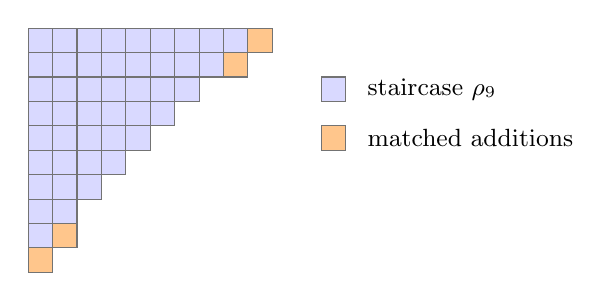
\begin{tikzpicture}[x=.31cm,y=-.31cm,every node/.style={font=\small}]
 \foreach \row/\width in {1/10,2/9,3/7,4/6,5/5,6/4,7/3,8/2,9/2,10/1}{
  \foreach \column in {1,...,\width}{
   \pgfmathtruncatemacro{\staircasecell}{\row+\column<=10}
   \ifnum\staircasecell=1
    \fill[blue!15] (\column-1,\row-1) rectangle (\column,\row);
   \else
    \fill[orange!45] (\column-1,\row-1) rectangle (\column,\row);
   \fi
   \draw[black!55] (\column-1,\row-1) rectangle (\column,\row);
  }
 }
 \fill[blue!15] (12,2) rectangle (13,3);
 \draw[black!55] (12,2) rectangle (13,3);
 \node[right] at (13.5,2.5) {staircase $\rho_9$};
 \fill[orange!45] (12,4) rectangle (13,5);
 \draw[black!55] (12,4) rectangle (13,5);
 \node[right] at (13.5,4.5) {matched additions};
\end{tikzpicture}
\caption{The degree-$49$ candidate with $M=9$, $r=2$, $b=1$, and
$s=1$. Its row and column lengths are both
$(10,9,7,6,5,4,3,2,2,1)$. The four added cells come in transposed
pairs, preserving self-conjugacy.}
\label{fig:candidate}
\end{figure}

When $r=0$, the candidate is the staircase itself, and
Theorem~\ref{thm:cyclic-input} already supplies all constituents.
For $r>0$ we give two sufficient support tests. For a target $\nu$,
write its column heights and row lengths as
\[
 h=(h_1,h_2,\ldots)=\nu^t,\qquad
 w=(w_1,w_2,\ldots)=\nu,
\]
with zeros appended. Both tests refer to the single square
$S^L\otimes S^L$ fixed above. We are free to interchange $h$ and $w$
by Lemma~\ref{lem:candidate}.

The coverage has four steps. A small first-four row or column sum is
handled by Proposition~\ref{prop:balance-four}. Otherwise the band
criterion covers every $M\ge22$ and all intermediate parameters apart
from the nineteen pairs in \eqref{eq:capacity-exceptions}; the exact
capacity check handles those pairs. Proposition~\ref{prop:finite-check}
handles all eligible degrees at most $64$, completing the small-index
remainder. The two finite checks thus have separate, explicitly bounded
roles.

\section{The band criterion}
\label{sec:band}

We use the parameters and the self-conjugate diagram $L$ from
\eqref{eq:candidate}, and write $K=2M-1$.  In particular,
$r=2b+s-1$.  The following criterion supplies constituents whose
diagrams have enough room for a path and its two attachments.

\begin{proposition}[Band criterion]\label{prop:band-test}
Let $M\ge9$, and let $\lambda\vdash |L|$ have column heights
$h_1\ge h_2\ge\cdots$ and row lengths $w_1\ge w_2\ge\cdots$,
with zeros appended.  Suppose that integers $d,q$ satisfy
$1\le d\le4$, $0\le q\le8$, and
\begin{equation}\label{eq:band-criterion}
 \sum_{i=1}^d w_i\ge K,\qquad
 dq+7+d\le K,\qquad
 \sum_{i=1}^q
      \max\left(0,\left\lfloor\frac{h_i-d}{2}\right\rfloor\right)
       \ge r.
\end{equation}
Then $S^\lambda$ occurs in $S^L\otimes S^L$.
\end{proposition}

The three inequalities have separate roles: the first gives room for
the path, the second reserves space at its endpoints, and the third
provides the even column heights needed for the attachments. We first
force the smaller cyclic triangle, then find nonzero path and attachment
contractions, and finally show that they combine without cancellation.
All alternating tensors use the conventions of
Section~\ref{sec:prelim}; changing the order of a block changes only its
overall sign.

\subsection{A forced triangle and a full induced quotient}

We first record the elementary induction fact used here and in the
balance constructions. It is the coordinate-sector principle of
\cite[Section~4]{SaxlCyclic}, applied to the marked alphabets of the
enlarged diagram.

\begin{lemma}[Induction from coordinate sectors]
\label{lem:sector-induction}
Let a finite group $G$ act transitively on a finite set $\Omega$.
Suppose a $G$-module has a direct-sum decomposition
$T=\bigoplus_{A\in\Omega}T_A$ with $gT_A=T_{gA}$.
Fix $D\in\Omega$, let $H$ be its stabilizer, and let $z\in T_D$.
Writing $A_0=\C[H]z$, the map
\[
 \C[G]\otimes_{\C[H]}A_0\longrightarrow\C[G]z,
 \qquad g\otimes a\longmapsto ga,
\]
is an isomorphism.  In particular, the cyclic module on the right is
the full induced module $\Ind_H^G A_0$.
\end{lemma}

\begin{proof}
Choose one representative $g_A$ with $g_AD=A$ for each $A\in\Omega$.
The source is the direct sum of the spaces $g_A\otimes A_0$.
Their images are $g_AA_0\subseteq T_A$, so the images for distinct
$A$ are linearly independent.  On each summand the displayed map is
injective, since $g_A$ acts invertibly.  Its image contains every
translate of $z$, proving surjectivity as well.
\end{proof}

Regard $L$ as its set $B$ of cells, with rows and columns indexed from
one.  Let $v_R,v_C$ be the alternating block tensors for its rows and
columns, respectively, and put
\[
 W_L=\C[S_B](v_R\otimes v_C).
\]
Both factors have type $L$, since $L$ is self-conjugate; hence
$W_L\subseteq S^L\otimes S^L$ after choosing the Specht
identifications.  Let
\[
 D=\{(i,j):i,j\ge1,\ i+j\le M-1\},\qquad F=B\setminus D.
\]
Thus $D$ is the staircase of order $M-2$, and
$|F|=K+2r$.

\begin{lemma}[Triangle quotient]\label{band:triangle-quotient}
There is a quotient of $W_L$ isomorphic to
\begin{equation}\label{eq:band-triangle-quotient}
 \Ind_{S_D\times S_F}^{S_B}
       (W_{M-2}\boxtimes U_F),
\end{equation}
where $W_{M-2}$ is the specified cyclic module in
Theorem~\ref{thm:cyclic-input}.  The module $U_F$ is generated by
the row and column block alternations on $F$, using an initial
alphabet on every remaining block.
Consequently, it suffices to find a diagram $\mu\subseteq\lambda$
of size $|F|$ such that $S^\mu$ occurs in $U_F$.
\end{lemma}

\begin{proof}
Set $\ell=M+b+s-1$, the largest row and column length of $L$.
The triangle $D$ has $t_i=\max(M-1-i,0)$ cells in row $i$
and in column $i$.  We will give each full row and column block
exactly this number of marked letters.
In each of the two alphabets $1,\ldots,\ell$, mark precisely
\[
 \{3,4,\ldots,M-1\}\cup\{M+b\}.
\]
There are $M-2$ marked letters.  The number of marked letters in
the initial alphabet of row or column $i$ is indeed $t_i$:
for the two largest blocks these counts are
$M-2,M-3$, and thereafter they are $M-4,M-5,\ldots,1,0,\ldots$.
The ordered unmarked alphabet is
$(1,2,M,\ldots,M+b-1)$, followed by $M+b+1$ if $s=2$.
The interval $M,\ldots,M+b-1$ is empty when $b=0$; in this case
the marked alphabet is $(3,\ldots,M)$ and the unmarked alphabet
is $(1,2)$ or $(1,2,M+1)$, respectively.  In every case each
block inherits an initial list in each of these two ordered
alphabets.
Project the pair-letter tensor space by retaining only those words
whose two letters at every position have the same marking status.
The projection commutes with permutations of positions.

For any retained term of $v_R\otimes v_C$, the set $A$ of marked
positions has row and column margins $(t_i)$.  For every $k$,
\[
 \sum_{i=1}^k t_i=\sum_j\min(k,t_j).
\]
Column $j$ can place at most $\min(k,t_j)$ marked cells in the
first $k$ rows.  Equality of the sums therefore gives equality in
every column.  Taking $k=t_j$ shows that, when $t_j>0$, all its
marked cells occupy the first $t_j$ rows.  Hence $A=D$.

Within each row or column block, the marked and unmarked positions
are now fixed.  Expanding that block's alternation gives the tensor
product of its marked and unmarked alternations, multiplied by one
fixed shuffle sign.  The two alphabets, each in its inherited order,
have initial lists on every block.  Thus, up to an overall sign, the
projected generator is
\[
 w_{M-2}\otimes u_F,
\]
where $w_{M-2}$ is exactly the row-column generator of
Theorem~\ref{thm:cyclic-input}, with its ordered alphabet relabeled,
and $u_F$ is the generator described in the statement.
The stabilizer $S_D\times S_F$ generates
$W_{M-2}\boxtimes U_F$ from this tensor.  To specify the sectors,
let $V_{\mathrm{mark}}$ and $V_{\mathrm{unmark}}$ be the pair-letter
spaces in which both letters are marked or both are unmarked,
respectively.  For $A\subseteq B$ with $|A|=|D|$, put
\[
 T_A=V_{\mathrm{mark}}^{\otimes A}\otimes
          V_{\mathrm{unmark}}^{\otimes(B\setminus A)}.
\]
These spaces have disjoint word bases, and $gT_A=T_{gA}$.
Lemma~\ref{lem:sector-induction} therefore identifies the entire
projected cyclic image with the full induced module in
\eqref{eq:band-triangle-quotient}, not merely with one of its
quotients.

For the last assertion, suppose $\mu\subseteq\lambda$.
Iterated branching implies that $S^\mu$ occurs on restriction of
$S^\lambda$ to $S_F$.  Decompose
$\Res_{S_D\times S_F}^{S_B}S^\lambda$ and then forget the $S_D$
action.  The occurrence just noted implies that some
$\alpha\vdash|D|$ satisfies $c_{\alpha,\mu}^{\lambda}>0$.
Theorem~\ref{thm:cyclic-input} supplies $S^\alpha$ in $W_{M-2}$.
Thus $S^\lambda$ occurs in the induced module in
\eqref{eq:band-triangle-quotient}, and hence in $W_L$ by complete
reducibility.
\end{proof}

\subsection{The path and its two attachments}

Write $\delta=s-1\in\{0,1\}$ and $E=(b+\delta,b)$, omitting
zero parts.  Each copy of $E$ has area $r$.
To decompose $F$, start with the boundary cells $i+j=M$ or $M+1$
in the staircase $B_M$.  They form a width-two path of length $K$.
Move its endpoint singletons from $(M,1)$ and $(1,M)$ to
$(\ell,1)$ and $(1,\ell)$, respectively.  More precisely, the
resulting path positions are $p_1,\ldots,p_K$, where
\begin{align*}
 p_1&=(\ell,1),&p_K&=(1,\ell),\\
 p_{2j}&=(M-j,j) &&(1\le j<M),\\
 p_{2j-1}&=(M+1-j,j) &&(2\le j<M).
\end{align*}
The northeastern attachment is
\[
 E_+=\{(1,j):M\le j\le\ell-1\}
       \cup\{(2,j):M\le j\le M+b-1\},
\]
with an interval interpreted as empty when its upper endpoint is
smaller than its lower endpoint.  Let $E_-$ be its transpose.
These sets are pairwise disjoint and exhaust $F$.
The attachment $E_+$ has shape $E$, and $E_-$ has the transposed
incidence pattern.

Along the path, the column pairs are
$(p_1,p_2),(p_3,p_4),\ldots,(p_{K-2},p_{K-1})$, with a column
singleton at $p_K$.  The row pairs are
$(p_2,p_3),(p_4,p_5),\ldots,(p_{K-1},p_K)$, with a row singleton
at $p_1$.  Only the first two column pairs and the last two row
pairs belong to blocks extended by attachment cells.

\begin{figure}[ht]
\centering
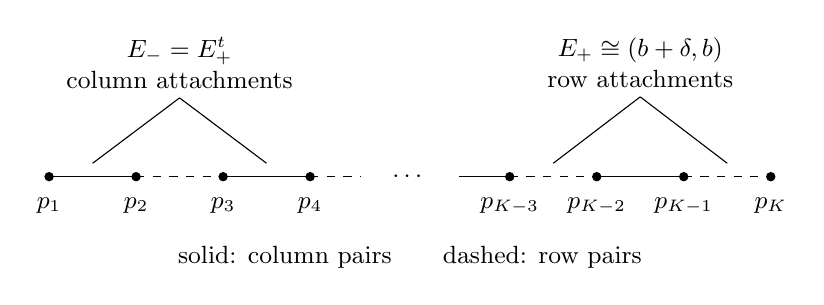
\begin{tikzpicture}[x=1.3cm,y=1cm, every node/.style={font=\small}]
 \foreach \name/\x/\lab in
   {a/0/{p_1},b/.85/{p_2},c/1.7/{p_3},d/2.55/{p_4},
    e/4.5/{p_{K-3}},f/5.35/{p_{K-2}},g/6.2/{p_{K-1}},h/7.05/{p_K}}
  {\coordinate (\name) at (\x,0);
   \fill (\name) circle (1.7pt);
   \node[below=4pt] at (\name) {$\lab$};}
 \draw (a)--(b); \draw[dashed] (b)--(c); \draw (c)--(d);
 \draw[dashed] (d)--(3.05,0);
 \node at (3.52,0) {$\cdots$};
 \draw (4,0)--(e);
 \draw[dashed] (e)--(f); \draw (f)--(g); \draw[dashed] (g)--(h);
 \node[align=center] (sw) at (1.275,1.45)
     {$E_-=E_+^t$\\column attachments};
 \draw (sw.south)--(.425,.17);
 \draw (sw.south)--(2.125,.17);
 \node[align=center] (ne) at (5.775,1.45)
     {$E_+\cong(b+\delta,b)$\\row attachments};
 \draw (ne.south)--(4.925,.17);
 \draw (ne.south)--(6.625,.17);
 \node at (3.525,-1.02)
     {solid: column pairs\qquad dashed: row pairs};
\end{tikzpicture}
\caption{Block-incidence schematic for $F$.  Each attachment extends
the two indicated pair blocks by $b+\delta$ and $b$ cells, respectively
(at the right, the outer pair receives $b+\delta$).
The displayed coordinates $p_i$ are defined in the text; the drawing
is not a geometric placement of the Young diagram.  Every path position
outside its first and last four belongs only to unextended blocks.}
\label{fig:band-attachments}
\end{figure}

Relabel the unmarked alphabet in increasing order, starting at one.
Let $P$ be the four-dimensional pair-letter space spanned by
$e_a\otimes e_c$ with $a,c\le2$.  Let
\[
 X_+=\Span\{e_a\otimes e_c:a>2,\ c\le2\},\qquad
 X_-=\Span\{e_a\otimes e_c:a\le2,\ c>2\},\qquad
 X=X_+\oplus X_-.
\]
Only letters available in the complement alphabet are included in
these spans.  There are $b+\delta$ letters above two, so
\[
 \dim X=4(b+\delta)\ge 4b+2\delta=2r.
\]
In particular, every extra diagram of size $2r$ fits this actual
alphabet; when $r=0$, both the diagram and $X$ are empty.
No cell of $F$ is simultaneously in one of its two long rows and
one of its two long columns, so every pair letter in $u_F$ lies in
$P\oplus X$.

\begin{lemma}[Separated contraction]\label{band:separated}
Retain from $u_F$ only terms using $P$ on the path, $X_+$ on $E_+$,
and $X_-$ on $E_-$.  The resulting tensor is, up to one nonzero
overall sign,
\begin{equation}\label{eq:band-separated}
 u_{\mathrm{path}}\otimes z_+\otimes z_-.
\end{equation}
Here $u_{\mathrm{path}}$ is the product of the two path block
alternations, with both endpoint singleton letters equal to one.
The tensors $z_+,z_-$ are the row-column alternating generators
for the two copies of $E$, with the long-block index shifted by two
and the two tensor layers interchanged for $E_-$.
\end{lemma}

\begin{proof}
In each extended block its two path positions must take its low
letters $1,2$, while its extra positions must take all remaining
letters.  These are prescribed sets of positions.  The alternation
therefore splits into an independent alternation on each set, with
a fixed shuffle sign.  Every other block belongs entirely to the
path or to one attachment.  Multiplying these factorizations proves
\eqref{eq:band-separated}.
\end{proof}

The selection in Lemma~\ref{band:separated} refers to fixed regions
of $F$ and need not commute with position permutations.
We will use the factorization inside a dual-polytabloid contraction:
the endpoint placement in the final proof will force precisely these
selected terms to survive.

\subsection{Contractions on an odd path}

For $t\ge0$, Brown, van Willigenburg, and Zabrocki
\cite[Corollary~4.1]{BWZ} proved that the square of $S^{(t+1,t)}$
contains exactly the partitions of $2t+1$ with at most four rows,
each with multiplicity one.  We need this support in a specified
cyclic path tensor, with any consecutive placement of the dual
columns.  The following proof extends the explicit contraction in
\cite[Section~5]{SaxlCyclic} to every odd length, including a single
position, and gives the common-basis conclusion needed for several
paths at once in the balance constructions.

\begin{lemma}[Odd-path support]\label{band:path-support}
Let $k=2t+1$ with $t\ge0$.  On positions $1,\ldots,k$, put
alternating pairs in the first layer on
$(2,3),(4,5),\ldots,(k-1,k)$ and the singleton letter $1$ at
position $1$.  In the second layer put alternating pairs on
$(1,2),(3,4),\ldots,(k-2,k-1)$ and the singleton letter $1$ at
position $k$.  Denote the resulting pair-letter tensor by $u$.

For every ordered list $a_1,\ldots,a_c$ with
$1\le a_i\le4$ and $\sum_i a_i=k$, place the columns of a dual
polytabloid consecutively along the path with these lengths.
There is a common ordered basis of $\Mat_2(\C)$ for which its
contraction with $u$ is nonzero.  In particular, the cyclic span of
$u$ contains every partition of $k$ with at most four rows.
For any finite collection of such paths and ordered column lists,
one common generic basis makes all their contractions nonzero.
\end{lemma}

\begin{proof}
Identify a pair-letter covector with a matrix $Y$ by evaluation
$Y(e_a\otimes e_c)=Y_{ac}$, and put
\[
 J=\begin{pmatrix}0&1\\-1&0\end{pmatrix}.
\]
Expanding the pair alternations and successively contracting the
indices along the path gives
\begin{align}
 \langle u,Y_1\otimes\cdots\otimes Y_k\rangle
 &=\bigl[Y_1JY_2^{\mathsf T}JY_3\cdots
                 JY_{k-1}^{\mathsf T}JY_k\bigr]_{11}\notag\\
 &=(-1)^t
   \bigl[Y_1\adj(Y_2)Y_3\cdots\adj(Y_{k-1})Y_k\bigr]_{11},
 \label{eq:band-path-contraction}
\end{align}
because $JY^{\mathsf T}J=-\adj(Y)$ for a two-by-two matrix.
The formula also holds for $k=1$, with no intervening factors.

Use the ordered matrix basis
\[
 M_1=I,\qquad
 M_2=Z=\begin{pmatrix}1&0\\0&-1\end{pmatrix},\qquad
 M_3=T=\begin{pmatrix}0&1\\1&0\end{pmatrix},\qquad M_4=J=ZT.
\]
The last three matrices are traceless, invertible, and pairwise
anticommuting.  Adjugation fixes $I$ and negates the other three.
For a segment of length $a\le4$ beginning at global position $p$,
write $D_j(Y)=Y$ for odd $j$ and $D_j(Y)=\adj(Y)$ for even $j$.
Its alternated matrix is
\[
 A_{a,p}=\sum_{\pi\in S_a}\sgn(\pi)
       D_p(M_{\pi(1)})\cdots D_{p+a-1}(M_{\pi(a)}).
\]
Let $e$ be the number of even positions in this segment, and let
$\epsilon=1$ when $p$ is even and $\epsilon=0$ otherwise.  Then
\begin{equation}\label{eq:band-segment}
 A_{a,p}=a!(-1)^{e-\epsilon}M_1\cdots M_a.
\end{equation}
Indeed, if $I$ occupies the local slot $j$, moving it there
contributes $(-1)^{j-1}$ to the permutation sign, while reordering
all remaining matrices contributes precisely their permutation
sign by anticommutation.  The adjugations contribute
$(-1)^{e-\epsilon_j}$, where $\epsilon_j$ records whether
$p+j-1$ is even.  Since
$\epsilon_j\equiv\epsilon+j-1\pmod2$, the total sign is
$(-1)^{e-\epsilon}$ for every summand.  This proves
\eqref{eq:band-segment}, whose right side is invertible.
For example, at length three the formula gives $-6J$ for both
starting parities: the canonical product is $IZT=J$, and
$e-\epsilon=1$ in either case.

Consequently, alternating independently within the prescribed
consecutive segments in \eqref{eq:band-path-contraction} gives
$(-1)^t[B]_{11}$, where $B$ is the ordered product of their
invertible matrices $A_{a,p}$.  Choose an eigenvector of $B$ with
nonzero eigenvalue $\beta$, and a matrix $Q\in\GL_2(\C)$ taking
it to the first coordinate vector.  Replace every $M_i$ by
$QM_iQ^{-1}$.  Since adjugation commutes with conjugation, the
new contraction is $(-1)^t[QBQ^{-1}]_{11}=(-1)^t\beta\ne0$.
The endpoint letters of $u$ have remained fixed throughout.

The dual tensor is a polytabloid for the partition with the
specified column lengths, regardless of their order along the
path.  Lemma~\ref{lem:dual-test} proves the support assertion.
For any one placement its contraction is a polynomial in the
entries of the common basis and is not identically zero by what
we just proved.  The nonvanishing loci of finitely many such
polynomials have nonempty intersection with the open set of
ordered bases, since $\GL_4(\C)$ is irreducible.  This proves the
last assertion.
\end{proof}

\subsection{The support of the two extra copies}

The path supplies the four-row component. We now determine enough
support in each attachment to supply every even-column diagram required
by the last inequality of Proposition~\ref{prop:band-test}.
The first step adapts the signed-average argument of
\cite[Section~3]{SaxlCyclic} to the two-row attachment.

\begin{lemma}[One extra copy]\label{band:one-extra}
Let $E=(b+\delta,b)$, where $b\ge0$ and $\delta\in\{0,1\}$,
and let $Z_E$ be the cyclic span of its row-column alternating
generator.  The sign twist $Z_E\otimes\sgn$ contains every
partition $\alpha\vdash 2b+\delta$ with at most four rows such
that all its row lengths are even when $\delta=0$, or exactly one
row length is odd when $\delta=1$.
\end{lemma}

\begin{proof}
The empty diagram is immediate, so assume $|E|>0$.
Let $p$ be its short-column alternating vector and $v$ its
long-row alternating vector.  These generate Specht modules of
types $E$ and $E^t$, respectively; denote them by
$V_p$ and $V_v$.  Put $G=S_{|E|}$ and $\varepsilon=\sgn$.
Let $H$ permute
positions within each short column, so that $hp=\sgn(h)p$.
Signed averaging of the product gives
\[
 \sum_{h\in H}\sgn(h)h(v\otimes p)
       =\left(\sum_{h\in H}hv\right)\otimes p.
\]
The first factor $v_0=\sum_{h\in H}hv$ is nonzero.  In fact the
word assigning letter $j$ to every cell of short column $j$ is
fixed by $H$ and has coefficient one in the row alternation $v$,
so its coefficient in $v_0$ is $|H|$.

Choose an abstract $G$-isomorphism
$\phi:V_v\otimes\varepsilon\longrightarrow V_p$, which exists
by sign conjugacy.  The $H$-alternating line of $V_p$ is unique:
\begin{align*}
 \dim\Hom_H(\varepsilon|_H,\Res_H^G V_p)
 &=\dim\Hom_G(\Ind_H^G\varepsilon|_H,V_p)\\
 &=\dim\Hom_G(\Ind_H^G\mathbf1,V_p\otimes\varepsilon)\\
 &=1.
\end{align*}
For the last equality, $H$ has block sizes given by $E^t$, and
$V_p\otimes\varepsilon\cong S^{E^t}$; this is the diagonal
multiplicity in Lemma~\ref{lem:young-support}.
Since $v_0$ is $H$-fixed,
$\phi(v_0\otimes\zeta)=cp$ for a nonzero sign-module vector
$\zeta$ and some $c\ne0$.  Reassociating the sign twist into
the first factor and then applying $\phi\otimes\mathrm{id}$
identifies $(V_v\otimes V_p)\otimes\varepsilon$ with
$V_p\otimes V_p$.  The image of $Z_E\otimes\varepsilon$
contains $cp\otimes p$, so it contains the cyclic span of
$p\otimes p$.

This is an isomorphism of abstract symmetric-group modules; it
does not change the physical long alphabet into a two-letter
alphabet.  It proves a support inclusion for the original
attachment module.  The subsequent contraction calculation may
therefore be made in the convenient realization of $p\otimes p$
on two copies of a two-dimensional alphabet.

Regroup the latter tensor by positions.  Each repeated short pair
is the symmetric tensor
\begin{equation}\label{eq:band-pair-form}
 H_0=e_{11}\otimes e_{22}+e_{22}\otimes e_{11}
       -e_{12}\otimes e_{21}-e_{21}\otimes e_{12}
\end{equation}
on the four-dimensional space with basis
$e_{ac}=e_a\otimes e_c$.  It is nondegenerate.  If $\delta=1$,
there is also the singleton vector $v_*=e_{11}$.

Suppose first that $\alpha$ has even rows.  Pair adjacent columns
of its dual tableau; the two columns in each pair have equal
height.  Place the $b$ position pairs of $H_0^{\otimes b}$
across corresponding rows of these paired columns.  Choose an
orthonormal basis of covectors for the form $H_0$.
In any nonzero term of the dual column alternations, the two
permutations on a paired column pair must match.  Their signs
therefore multiply to one.  A paired column pair of height $a$
contributes $a!$, so the entire contraction is nonzero.

When $\alpha$ has exactly one odd row, adjacent columns have
equal heights except for a single paired column pair of heights
$a,a-1$.  Put the singleton at the bottom of its longer column
and place the remaining position pairs across corresponding
rows.  In that exceptional pair, matching the other covectors
forces the singleton to receive the $a$th basis covector.
The contribution is $(a-1)!$ times its evaluation on $v_*$.
Choose the orthonormal basis so that this evaluation is nonzero;
this is possible since $v_*\ne0$, by permuting the members of
any orthonormal basis if necessary.  The covectors span the dual
space, so at least one evaluates nontrivially on $v_*$.  The other
column pairs contribute their positive factorials as before.  Thus this
contraction is also nonzero.  The height bound four ensures that
all covectors used belong to the available basis.
Lemma~\ref{lem:dual-test} completes the proof.
\end{proof}

\begin{lemma}[Two extra copies]\label{band:two-extras}
The cyclic span of $z_+\otimes z_-$ on $E_+\sqcup E_-$ contains
every diagram $\eta\vdash 2r$ whose column heights are even and
whose number of columns is at most eight.
\end{lemma}

\begin{proof}
The alphabets $X_+$ and $X_-$ are disjoint.  The same coordinate
sector argument as in Lemma~\ref{lem:sector-induction} identifies
this cyclic module with the full induction of the two local
cyclic modules.  Transposing $E$ merely interchanges its two
tensor layers, so both local modules are isomorphic to $Z_E$.

Put $\theta=\eta^t$.  Its rows have even lengths and
there are at most eight of them.  Group its columns in adjacent
pairs, and let $j_1,\ldots,j_a\le8$ be the heights of those
double columns.  Thus
\[
 \theta=(2^{j_1})+\cdots+(2^{j_a}),\qquad
 j_1+\cdots+j_a=r,
\]
where addition of diagrams is rowwise.
For each $j$, splitting its height as $j=u+v$ gives
\[
 c_{(2^u),(2^v)}^{(2^j)}>0.
\]
Indeed the corresponding single-column coefficient is positive,
and Lemma~\ref{lem:lr-addition} applies twice.
Choose $u=\lfloor j/2\rfloor$, $v=\lceil j/2\rceil$, allowing
their interchange.  Both are at most four.

If $r$ is even, the number of odd $j_i$ is even.  Alternate the
orientation of the split on these odd heights.  The resulting
two rowwise sums $\alpha,\beta$ each have size $r$, at most four
rows, and all row lengths even.  Repeated use of
Lemma~\ref{lem:lr-addition} gives $c_{\alpha,\beta}^{\theta}>0$.

If $r$ is odd, reserve one odd height $j=2k+1$.  For this double
column take the two equal-area shapes
\[
 \kappa=(2^k,1),\qquad
 c_{\kappa,\kappa}^{(2^{2k+1})}>0.
\]
The displayed coefficient follows from rectangle complement
duality in the Littlewood--Richardson rule, since $\kappa$ is
its own rotated complement in this rectangle.  Equivalently,
fill the single remaining cell in row $k+1$ by $1$, and in
each later row $k+t$, for $2\le t\le k+1$, put $t-1,t$ from
left to right.  This is a Littlewood--Richardson filling with
content $\kappa$, including the case $k=0$.
There are now an even number of odd heights left; alternate their
orientations as above.  Their combined area is $2(r-j)$, and
the balanced split gives $r-j$ cells to each factor; the reserved
copy of $\kappa$ adds $j$ cells to each.  Each final factor thus
has size $r$, at most four rows, and exactly one odd row, since
the remaining rowwise summands have only even rows.
Here $k+1\le4$ because $j\le8$.  At the endpoints this includes
$r=j=1$, with $\kappa=(1)$, and $j=7$, with
$\kappa=(2,2,2,1)$ of size seven and height four.
Again horizontal addition gives a positive coefficient for
$\theta$.

Lemma~\ref{band:one-extra} supplies both resulting factor
partitions in $Z_E\otimes\sgn$.  Induction commutes with a sign
twist, since the restriction of the sign character is the product
of the two local sign characters.  Thus $\theta$ occurs in the
sign twist of the two-copy module, and $\eta$ occurs in the
untwisted module.  The case $r=0$ is the empty tensor and obeys
the same conclusion.
\end{proof}

\subsection{Attaching without cancellation}

The local contractions are now available. The remaining issue is their
interaction: an elongated dual column could in principle mix path and
attachment covectors. The endpoint clearance in the criterion allows us
to place the covectors so that all mixed assignments vanish.

\begin{proof}[Proof of Proposition~\ref{prop:band-test}]
Choose an even list $e_1\ge\cdots\ge e_t>0$, with $t\le q$,
such that
\begin{equation}\label{eq:band-extra-capacities}
 \sum_{i=1}^t e_i=2r,\qquad e_i\le h_i-d.
\end{equation}
For example, fill the capacities
$\max(0,\lfloor(h_i-d)/2\rfloor)$ from left to right until their
sum reaches $r$, then double the filled amounts and discard zeros.
The capacities decrease, so the resulting positive list decreases.
When $r=0$, take the empty list and $t=0$.

Put $d$ path cells in each of these $t$ columns.  The total
available path capacity is
\[
 \sum_i\min(d,h_i)=\sum_{i=1}^d w_i\ge K.
\]
Fill further columns, in order, with at most $\min(d,h_i)$ path
cells until the path total is exactly $K$.  This produces a
decreasing column list for a path diagram $\pi$; its first $t$
columns have height $d$, and every column has height at most $d$.
Increase the first $t$ column heights by $e_i$ to form $\mu$.
By construction $\mu\subseteq\lambda$ and $|\mu|=K+2r$.
Call the first $t$ path columns chosen and all other nonempty
path columns unchosen.

The total length of unchosen path columns is
\[
 K-dt\ge K-dq\ge7+d.
\]
Order some of these columns first, stopping when their total
length first reaches four.  Each has length at most $d$, so
this prefix has length between four and $3+d$.  Put the chosen
columns next, then all remaining unchosen columns.  The final
group has length at least four.  Lay these columns consecutively
along the path in this order.  All path positions in a chosen
column now lie outside the first and last four path positions;
their original row and column blocks are consequently unextended.

By Lemma~\ref{band:path-support}, there is an ordered basis
$N_1,\ldots,N_4$ of $P^*$ for which the path polytabloid using
these consecutive columns has nonzero contraction with
$u_{\mathrm{path}}$.  Only its first $d$ basis covectors are used.
Let $\eta$ be the extra diagram with column heights
$e_1,\ldots,e_t$.  Lemma~\ref{band:two-extras} and
Lemma~\ref{lem:dual-test} give an ordered basis
$Q_1,\ldots,Q_{\dim X}$ of $X^*$ and a placement of its dual
columns on the extra positions for which the contraction with
$z_+\otimes z_-$ is nonzero.  The empty case has contraction one.
This applies the dual test to the actual extra tensor in $X$;
the abstract Specht identification in
Lemma~\ref{band:one-extra} was used only to prove its support.
The $Q_j$ may mix $X_+^*$ and $X_-^*$, and an extra dual column
may use positions from both attachments.  Neither is a
restriction: assign each such extra column to a chosen path
column with the corresponding height $e_i$.

Extend these covectors by zero on the other summand of $P\oplus X$.
Use the single ordered flag beginning
\[
 N_1,\ldots,N_d,Q_1,\ldots,Q_{\dim X},
       N_{d+1},\ldots,N_4.
\]
For every chosen column, adjoin its extra column of $e_i$ positions
below its $d$ path positions.  The other columns have only their
path positions.  This is a placement of the column blocks of a
dual polytabloid of shape $\mu$.

We check all terms of its alternating expansion.  At each chosen
path position, both row and column block lengths in the
complement generator $u_F$ are at most two (the assertion is
about its remaining blocks, not their lengths in $L$).
The pair letter therefore belongs to $P$ and is annihilated by
every $Q_j$.  The $d$ path positions in such a column must use
all its $N$-covectors, leaving precisely its $Q$-covectors on its
extra positions.  There are exactly $d$ such $N$-covectors, so
none can be assigned to an extra slot.  Unchosen columns already have only
$N$-covectors.  Thus every surviving assignment uses $P$ on the
entire path and $X$ on all extra positions.  On $E_+$ the only
possible such letters lie in $X_+$, and on $E_-$ they lie in
$X_-$.  No additional mixed assignment survives.

We may consequently replace $u_F$ in this contraction by its
separated tensor from Lemma~\ref{band:separated}.  In every
elongated dual column the surviving permutations also factor:
they permute the $N$-covectors among its path slots and the
$Q$-covectors among its extra slots, with a fixed cross sign.
Order the path slots before the extra slots to make that sign
one.  The full contraction is therefore, up to the fixed sign
in \eqref{eq:band-separated},
\[
 \langle u_{\mathrm{path}},\text{path polytabloid}\rangle
 \;\langle z_+\otimes z_-,\text{extra polytabloid}\rangle,
\]
and both factors are nonzero.  Lemma~\ref{lem:dual-test} gives
$S^\mu$ in $U_F$.  Finally, $\mu\subseteq\lambda$, so
Lemma~\ref{band:triangle-quotient} proves the proposition.
\end{proof}

\section{Balance tests}
\label{sec:balance}

Retain the self-conjugate candidate $L$ in
Equation~\eqref{eq:candidate}. For this second support test we use the
full square $S^L\otimes S^L$, with both factors realized by
column-alternating tensors on the same column blocks. Put
\[
 c=2b+2,\qquad T=2M-1+r.
\]
Thus $c$ is the total size of the columns of length two, and $T$ is
the sum of the two largest column lengths. We prove that a target
occurs whenever its first four column heights have sum at most
$2M-2$. The local components below supply balanced lists of
trivial-factor sizes, whose induced support is tested by Young's
rule. We then establish an additional three-row support statement
for the bounded capacity checks.

For reference, write
\begin{align*}
 \mathcal H_j(t)&=\{\nu\vdash t:\ell(\nu)\le j\},\\
 \mathcal E_j(t)&=\{\nu\in\mathcal H_j(t):
                         \text{every row length of $\nu$ is even}\}.
\end{align*}
If $t$ is even, let $\mathcal O_4(t)$ be the members of
$\mathcal H_4(t)$ having an odd-height column.  Finally,
$\mathcal P_3(c,s)$ denotes the partitions with at most three rows
obtained from a member of $\mathcal E_3(c)$ by adding a horizontal
strip of size three and then a horizontal strip of size $s$.
All support statements below mean inclusion, without any assertion
about multiplicities.

\subsection{Separating components by output values}

Use independent ordered alphabets in the two Specht factors.
A pair of letters $(a,a')$ has output
\[
 z(a,a')=a+a'-1.
\]
For a collection $B$ of column blocks on a position set $D_B$, let
$v_B$ be their alternating tensor and put
$Y_B=\C[S_{D_B}]v_B$. By Equation~\eqref{eq:block-specht}, this is
the Specht module whose column lengths are the sizes of the blocks
in $B$. Realize both copies of $Y_B$ on $D_B$. Every pair word
occurring in their tensor square has the same number of positions
and the same output sum:
\begin{equation}
 d_B=\sum_{A\in B}|A|,
 \qquad
 \sigma_B=\sum_{A\in B}|A|^2.
 \label{bal:fixed-sums}
\end{equation}
Indeed, a block of length $k$ uses $1,\ldots,k$ once in each
factor, so its output sum is $2(1+\cdots+k)-k=k^2$. Permuting
positions within $D_B$, independently in the two layers, preserves
these totals.

\begin{lemma}[Separation by sizes and sums]
\label{lem:balance-separation}
Partition the column blocks of $L$ into collections
$B_1,\ldots,B_v$ on disjoint position sets $D_1,\ldots,D_v$,
using the same blocks in both factors. Suppose $I_1,\ldots,I_v$ are
nonempty sets of integers with every element of $I_i$ smaller than
every element of $I_{i+1}$. Let $W_i$ be the image of
$Y_{B_i}\otimes Y_{B_i}$ under the coordinate projection retaining
words all of whose outputs lie in $I_i$. Then the support of
$S^L\otimes S^L$ contains the support of
\[
 \Ind_{S_{d_{B_1}}\times\cdots\times S_{d_{B_v}}}^{S_n}
       (W_1\boxtimes\cdots\boxtimes W_v).
\]
\end{lemma}

\begin{proof}
In the full pair-word space, retain precisely the words whose
outputs lie in $\bigcup_i I_i$ and for which the outputs in $I_i$
have cardinality $d_{B_i}$ and sum $\sigma_{B_i}$, for every $i$.
This coordinate projection commutes with all position permutations.

Consider a word from the tensor product with the prescribed
component positions. The positions in $D_1$ have
cardinality $d_{B_1}$ and sum $\sigma_{B_1}$ by
Equation~\eqref{bal:fixed-sums}.  In a retained word, the positions
whose outputs lie in $I_1$ have the same cardinality and sum.
If these two sets of positions differed, the positions in the first
set but not the second would all have larger outputs than the
positions in the second but not the first.  The two set differences
have equal positive cardinality, contradicting equality of their
sums.  The two sets therefore agree.  Remove them and repeat the
argument for $I_2$, and then successively for every range.

It follows that the global projection on these prescribed positions
is the tensor product of the local projections. More explicitly,
write $v_i=v_{B_i}$, $Y_i=Y_{B_i}$, and
$H=\prod_i S_{D_i}$. Inside either Specht factor,
\[
 \C[H](v_1\otimes\cdots\otimes v_v)
       =Y_1\boxtimes\cdots\boxtimes Y_v\subseteq S^L.
\]
Taking its tensor square gives the actual subspace
$\boxtimes_i(Y_i\otimes Y_i)$ in $S^L\otimes S^L$: the two
layers can be generated independently. The symmetric groups act
diagonally on each local square and on the global square. The
restriction of the global projection is $\bigotimes_i P_i$, where $P_i$ is the
local projection.  Its image is therefore the full outer product
$W_1\boxtimes\cdots\boxtimes W_v$.
Different ordered placements of these components have disjoint
coordinate supports, distinguished by which positions have outputs
in each $I_i$.  Their translates therefore give the full induced
module in the statement.  Since an equivariant image cannot acquire
a new irreducible type, the result follows.
\end{proof}

The local support guarantees proved in the following subsections are
summarized in Table~\ref{bal:local-table}. The entries concerning the largest
two lengths use $q=M+b-1$.  When $s=1$, their lengths are $q+1,q$;
when $s=2$, their lengths are $q+2,q$.

\begin{table}[htbp]
\centering
\small
\renewcommand{\arraystretch}{1.25}
\begin{tabular}{@{}p{0.25\linewidth}p{0.15\linewidth}p{0.19\linewidth}p{0.29\linewidth}@{}}
\hline
Column blocks & Total size & Allowed outputs
    & Guaranteed support\\
\hline
$a$ copies of $k$ & $ak$ & $\{k\}$ & $(ak)$\\
$u,u-1$ & $2u-1$ & $[u-1,u]$ & $\mathcal H_4(2u-1)$\\
$q+2,q$ & $2q+2$ & $[q,2q+3]$ & $\mathcal O_4(2q+2)$\\
$b+1$ copies of $2$ & $c$ & $\{2\}$ & $\mathcal E_2(c)$\\
$3$, $b+1$ copies of $2$, and $s$ copies of $1$
    & $c+3+s$ & $[1,3]$ & $\mathcal P_3(c,s)$\\
\hline
\end{tabular}
\caption{Local projected supports.  Neighboring intervals in a
packing are chosen disjoint before applying
Lemma~\ref{lem:balance-separation}.}
\label{bal:local-table}
\end{table}

After applying Lemma~\ref{lem:balance-separation}, transitivity
of induction permits us to combine selected factors in any order.
In particular, the big pair can be combined with the singleton
component even though their output ranges are not adjacent.

\subsection{Coordinate functionals and path components}

We first explain exactly how a surviving word coordinate supplies
a path vector after the two sign twists.

\begin{lemma}[The sign-twisted coordinate line]
\label{bal:coordinate-line}
Let $X=S^\mu$ be realized by column-alternating vectors in the word
space of content $\mu=(\mu_1,\mu_2,\ldots)$.  For a word $a$ of
this content, let $R_a$ permute separately the positions carrying
each equal letter.  The restriction $\epsilon_a|_X$ of its
coordinate functional is nonzero.  Under
$X^*\otimes\sgn\simeq S^{\mu^t}$, its line is the
line of the column-alternating vector on the equal-letter blocks
of $a$, whose lengths are $\mu_1,\mu_2,\ldots$.
\end{lemma}

\begin{proof}
For the row-constant word of a tableau, its coefficient in the
tableau's column-alternating vector is one: only the identity in
each column stabilizes that word.  Hence its coordinate restriction
is nonzero.  Every other word of the same content is a position
translate, which proves nonvanishing in general.

The restricted coordinate is $R_a$-invariant. Young's rule and
Frobenius reciprocity give
\[
 \dim (X^*)^{R_a}=1,
\]
using the diagonal multiplicity in Lemma~\ref{lem:young-support}.
After twisting by sign, this becomes the unique line on which
$R_a$ acts by its sign character.  The nonzero alternating vector
on the equal-letter blocks is such a vector, and its column
lengths are the parts of $\mu$; it therefore belongs to
$S^{\mu^t}$.  This identifies the two lines.
The identification is equivariant, so translating a word changes
the identification only by the corresponding sign and the
position translate.
\end{proof}

In a tensor square, these two sign twists cancel. To make the
passage through a projection explicit, let
$P:X\otimes X\longrightarrow W$ be a local coordinate projection
onto its image. Its dual embeds $W^*$ in $(X\otimes X)^*$.
For a surviving pair word, its coordinate functional $\epsilon$
satisfies $\epsilon(Pz)=\epsilon(z)$, so its restriction belongs
to this embedded copy of $W^*$. Lemma~\ref{bal:coordinate-line}
identifies it with a nonzero multiple of the product of the two
alternating vectors on its equal-letter blocks. Its entire
position-permutation span remains in $W^*$. Finding a path among
these products therefore proves support in $W$ itself, since
complex Specht modules are self-dual. In the next two lemmas, zero
column lengths are omitted.

\begin{lemma}[Neighboring lengths]
\label{bal:neighboring}
For every integer $u\ge1$, the local component with column lengths
$u,u-1$, projected to
outputs in $[u-1,u]$, contains every type in
$\mathcal H_4(2u-1)$.
\end{lemma}

\begin{proof}
Its content is $(2^{u-1},1)$.  The equal-letter blocks thus consist
of $u-1$ pairs and one singleton in each layer.  Arrange the two
pairings as one odd path.  From its first-layer singleton, label
that singleton $u$, and label the successive first-layer pairs
$u-1,u-2,\ldots,1$.  Label the second-layer pairs, in path order,
$1,2,\ldots,u-1$, and label its terminal singleton $u$.
At the path positions the outputs are alternately $u$ and $u-1$,
with output $u$ at both ends.

The pair word survives the stated projection.  By
Lemma~\ref{bal:coordinate-line}, its coordinate functional gives
the odd-path tensor in the sign-twisted dual square.  The twists
cancel, and Lemma~\ref{band:path-support} gives every partition
with at most four rows.  Consequently all these types occur in
the projected component.
\end{proof}

\begin{lemma}[The two-path component]
\label{bal:two-paths}
For every integer $q\ge0$, the component with column lengths
$q+2,q$, projected to outputs
in $[q,2q+3]$, contains $\mathcal O_4(2q+2)$.  If $q\ge3$,
inducing this support together with a trivial representation of
size two contains every member of $\mathcal H_4(2q+4)$.
\end{lemma}

\begin{proof}
The content is $(2^q,1,1)$.  In each layer there are pair labels
$1,\ldots,q$ and singleton labels $q+1,q+2$.
For any $0\le p\le q$, make odd paths of sizes $2p+1$ and
$2(q-p)+1$.  On the first path use first-layer pair labels
$1,\ldots,p$ and second-layer pair labels $q-p+1,\ldots,q$;
on the second path use the complementary intervals.  In path
order, the first-layer pairs decrease and the second-layer pairs
increase.  Give the first path the initial first-layer singleton
$q+1$ and terminal second-layer singleton $q+2$, and the second
path the remaining singletons.

Internal outputs are $q$ or $q+1$.  Endpoint outputs are at least
$q$, and all outputs are at most $2q+3$.  If one path is a
singleton, its two singleton labels satisfy the same bounds.
The resulting pair word therefore survives the projection, and
Lemma~\ref{bal:coordinate-line} identifies its coordinate with
the product of the two path tensors.

Let $\nu\in\mathcal O_4(2q+2)$.  Since its size is even, it has
an even positive number of odd-height columns.  Divide its columns
into two groups, each of odd total size.  These totals are
$2p+1$ and $2(q-p)+1$ for an allowed $p$.  Arrange each group's
columns consecutively on the corresponding path.  By
Lemma~\ref{band:path-support}, each contraction is a nonzero
polynomial in a common ordered basis of the pair-letter dual
space. Their product is also nonzero,
so a common generic ordered basis gives a nonzero contraction of the
two-path tensor with the dual tableau of $\nu$.  This proves the
first assertion.

For the second assertion, let $\eta\in\mathcal H_4(2q+4)$.
It has width greater than two when $q\ge3$.  We claim that some
removable horizontal two-strip leaves an odd-height column.
If $\eta$ has no odd-height columns, removing any horizontal
two-strip creates two.  If it has at least four, such a strip
cannot remove all of them.  If it has exactly two, its width
ensures that an even-height column also exists.  Remove one cell
from an odd-height column and one from an even-height column,
choosing the rightmost column of each selected height.  Their
heights are different, and these removals preserve the weakly
decreasing order of column heights.  This is a horizontal
two-strip and leaves two odd-height columns.  Pieri now proves
the desired containment.
\end{proof}

For the candidate diagram, the big component has $T$ positions.
When $s=1$, Lemma~\ref{bal:neighboring} supplies
$\mathcal H_4(T)$.  When $s=2$, its two singleton columns can
supply a trivial representation of size two at output one;
Lemma~\ref{lem:balance-separation} and
Lemma~\ref{bal:two-paths} then supply $\mathcal H_4(T+2)$.
The big component's outputs are at least $M-1$ in both cases.

\subsection{Symmetric pairs and short strips}

The path calculations handle the long columns. For the short-column
components we use a direct fact about repeated symmetric tensors.
Its polynomial-module conclusion is Littlewood's classical even-row
decomposition of symmetric powers of a symmetric square
\cite[Chapter~I, Section~5, Example~5(a); Appendix~A, Section~7,
Example~(1)]{Macdonald}.
The explicit contraction below also detects the prescribed tensor,
which is what our coordinate projection requires.

\begin{lemma}[Repeated symmetric pairs]
\label{bal:even-rows}
Let $m\ge0$ be an integer, let $E$ have dimension $j$, and let
$H\in\Sym^2 E$ be
nondegenerate.  The position-permutation span of
$H^{\otimes m}\in E^{\otimes 2m}$ contains every member of
$\mathcal E_j(2m)$.  Moreover, the polynomial $\GL(E)$-module
$\Sym^m(\Sym^2 E)$ contains the Schur module of each such
partition.
\end{lemma}

\begin{proof}
Choose an orthonormal basis for $H$, so
$H=\sum_{i=1}^j e_i\otimes e_i$.  A diagram with even row lengths
has its columns paired into equal-height pairs.  Place the two
positions of each copy of $H$ in corresponding cells of two
paired columns.  Contract against the usual column-alternating
dual tensor.  For a pair of columns of height $h$, the two
permutations must agree, their signs multiply to one, and their
contribution is $h!$.  The entire contraction is the nonzero
product of these factorials.  Lemma~\ref{lem:dual-test} proves
the first statement.

For the second, use the natural embedding of
$\Sym^m(\Sym^2 E)$ into $E^{\otimes 2m}$ with the $m$ pairs
of positions fixed, and choose the dual tableau placements as
above.  The same contraction proves that this $\GL(E)$-stable
subspace has a nonzero projection to the indicated Schur-Weyl
isotypic space.  Complete reducibility then gives the required
Schur module.
\end{proof}

An isolated length-$k$ block, projected to constant output $k$,
has the pair labels $(a,k+1-a)$ for $1\le a\le k$.  Reversing
one block's labels shows that all terms in the projected tensor
have the same sign.  It is a nonzero symmetric tensor and hence
supplies the trivial type of size $k$.  For several equal-length
blocks, the projected product still has coefficients of one
common sign.  Its full position average is nonzero, supplying
the trivial type of their total size.  This proves the first
row of Table~\ref{bal:local-table}.

On an aligned length-two block, projection to constant output two
gives, up to a common nonzero scalar,
\[
 e_{12}\otimes e_{21}+e_{21}\otimes e_{12}.
\]
This is a nondegenerate symmetric form on the two-letter space
$\Span(e_{12},e_{21})$.  Thus $b+1$ such blocks supply
$\mathcal E_2(c)$ by Lemma~\ref{bal:even-rows}.

\begin{lemma}[An odd horizontal strip]
\label{bal:odd-strip}
Let $c$ be positive and even, and let $x\in\{1,3\}$ with
$x\le c$.  Inducing the support $\mathcal E_2(c)$ with the
trivial representation of size $x$ supplies
$\mathcal H_2(c+x)$.
\end{lemma}

\begin{proof}
Write a target as $(\alpha,\beta)$, allowing $\beta=0$.
A precursor of size $c$ with even row lengths has the form
$(c-y,y)$ with $y$ even.  The horizontal-strip interlacing
conditions are precisely
\begin{equation}
 \max(0,\beta-x)\le y\le\min(\beta,c-\beta).
 \label{bal:parity-interval}
\end{equation}
The upper bound is at most $c/2$, so this also guarantees that
the precursor is a partition.  If the interval contains zero,
choose $y=0$.  Otherwise its lower endpoint is $\beta-x>0$.
When $\beta\le c/2$, its length is $x\ge1$.  When
$\beta>c/2$, its length is
$c+x-2\beta=\alpha-\beta$, a positive integer because
$c+x$ is odd.  The interval therefore contains an even integer.
Pieri gives the assertion.
\end{proof}

In our applications, the size-one strip is a singleton column
at output one, and the size-three strip is the length-three
block at output three.  These ranges are disjoint from output
two, so Lemma~\ref{lem:balance-separation} justifies the required
inductions.

\subsection{The first-four-column bound}

We now combine the local path and symmetric-pair supports. The aim is
to replace each component by a list of trivial-factor sizes and then
verify Young's dominance inequalities for the entire target.

For positive integers $t,j$, let $\operatorname{pack}(t,j)$
be the list of $j$ integers whose entries differ by at most one
and sum to $t$; zero entries, if any, are omitted.  Young's rule
implies that the support obtained by inducing trivial factors of
these sizes is exactly $\mathcal H_j(t)$.  Indeed, every partition
of $t$ with at most $j$ rows dominates the balanced $j$-part
partition, whereas a partition with more than $j$ rows fails
its $j$th dominance inequality.  Thus a local component supplying
$\mathcal H_j(t)$ may contribute $\operatorname{pack}(t,j)$
to a list of trivial-factor sizes for a support calculation.

\begin{proposition}[The balance bound]
\label{prop:balance-four}
Assume $M\ge9$, and let $h_1\ge h_2\ge\cdots$ be the column
heights of $\nu\vdash n$.  If
\begin{equation}
 \sum_{i=1}^4 h_i\le2M-2,
 \label{bal:four-small}
\end{equation}
then $S^\nu$ occurs in $S^L\otimes S^L$.
The same conclusion holds if Equation~\eqref{bal:four-small}
holds for the column heights of $\nu^t$.
\end{proposition}

\begin{proof}
Use the big pair, together with the two singleton columns when
$s=2$, to contribute four balanced parts of total $T+2(s-1)$.
When $s=1$, retain its singleton column as a separate part one.
If $c\le M$, use the length-two columns to contribute the single
part $c$.  Pair the middle lengths $3,\ldots,M-2$ consecutively,
leaving their smallest member alone if their number is odd.
Each paired pair of neighboring lengths contributes four balanced
parts by Lemma~\ref{bal:neighboring}, and an unpaired length
contributes itself.

If $c>M$, use the length-three block with the length-two blocks.
Lemma~\ref{bal:odd-strip} contributes two balanced parts of total
$c+3$, and now pair the remaining middle lengths $4,\ldots,M-2$
in the same fashion.  All output ranges used are disjoint:
the singletons have output one, the length-two and length-three
constructions use outputs two and three, a middle neighboring
pair uses the interval between its two lengths, and the big
pair uses outputs at least $M-1$.  Apply
Lemma~\ref{lem:balance-separation} first to these separate
components.  Then reassociate induction to combine the big
pair with the output-one singleton component when $s=2$, and
to combine the output-two and output-three components when
$c>M$.  The local support statements above now validate the
specified packing; no disconnected output range is treated
as a single component in the separation lemma.
Call the resulting list of parts $A$; its sum is $n$.

We record two uniform bounds:
\begin{equation}
 |A|\ge2M-5,
 \qquad \max A\le M+1.
 \label{bal:packing-bounds}
\end{equation}
A run of $p$ middle lengths contributes
$2p-(p\bmod2)\ge2p-1$ parts.  If $c\le M$, there are
$p=M-4$ middle lengths and at least five other parts, giving
at least $2M-4$ parts in total.  If $c>M$, then $M$ must be
even: for odd $M$, the bound $r\le M/2$ gives
$c\le r+2\le M/2+2<M$.  In the even case, $p=M-5$ is odd,
so the middle contribution is $2M-11$, and the big and short
components contribute at least six more parts.  This proves
the first bound.

Untouched lengths and balanced middle parts are at most $M$.
The largest big-component part is at most
\[
 \left\lceil\frac{T+2}{4}\right\rceil
 \le \left\lceil\frac{7M/2+3}{4}\right\rceil
 \le M+1,
\]
using $r\le3M/2+2$.  In the exceptional case $c>M$, the
largest short-component part is
\[
 \left\lceil\frac{c+3}{2}\right\rceil
   =\left\lfloor\frac r2\right\rfloor+3
   \le\left\lfloor\frac{3M}{4}\right\rfloor+4
   \le M+1.
\]
The last inequality holds for even $M\ge10$: it is equality
at $M=10$, and follows from $3M/4+4\le M+1$ for $M\ge12$.
This proves the second bound in
Equation~\eqref{bal:packing-bounds}.  In particular,
\begin{equation}
 \frac{n}{\max A}\ge\frac{N_M}{M+1}
      =\frac M2>\frac{2M-2}{4}.
 \label{bal:average-bound}
\end{equation}

We verify the inequalities of Lemma~\ref{lem:young-support}.
The target has at least four columns, since otherwise
Equation~\eqref{bal:four-small} would give
$n\le2M-2<N_M$.  Consequently $h_1\le2M-5$, and the first
inequality follows from $P_A(1)=|A|$.  The four big-component
parts are each at least two, so
\[
 P_A(2)\ge |A|+4\ge2M-1.
\]
This proves the inequalities for prefixes two and three as well.

For $k\ge4$, decreasing column heights and
Equation~\eqref{bal:four-small} imply
\[
 \sum_{i=1}^k h_i\le
       \min\left(n,\frac{k(2M-2)}4\right).
\]
Writing $B=\max A$, the termwise bound
$\min(k,a)\ge ka/B$ for $k\le B$ gives
\[
 P_A(k)\ge \min\left(n,\frac{kn}{B}\right).
\]
Equation~\eqref{bal:average-bound} proves every remaining
dominance inequality.  The constructed support therefore contains
$S^\nu$.  Finally, since $L$ is self-conjugate, its square
is invariant under sign twist, so the same conclusion follows
from the condition on $\nu^t$.
\end{proof}

\subsection{A three-row component}

The following construction is independent of the big pair and
will be used in the cases $M=10,12,14$.

\begin{proposition}[The short three-row component]
\label{prop:three-row}
Group the length-three block, the $b+1$ length-two blocks, and
the $s$ singleton blocks in both layers, and project to outputs
in $[1,3]$.  The resulting module contains every partition in
$\mathcal P_3(c,s)$.
This component can be induced independently with components on
the remaining lengths $4,\ldots,M-2$ and with the big pair.
\end{proposition}

\begin{proof}
Align corresponding blocks in the two layers and use pair letters
$e_{aa'}$.  Set
\[
 p=e_{11},\quad q=e_{22},\quad u=e_{12},\quad v=e_{21},
 \qquad a=e_{13},\quad d=e_{31}.
\]
These six pair letters form a basis of the space of outputs at
most three.  Each aligned length-two block contributes
\begin{equation}
 H=p\otimes q+q\otimes p-u\otimes v-v\otimes u.
 \label{bal:four-form}
\end{equation}
Each singleton contributes $p$.  The length-three block has
fixed output sum nine; since all its outputs are at most three,
they must all equal three.  Its contribution is, up to a nonzero
scalar, the full symmetrization of $a,d,q$.  Thus the projected
module contains the position orbit of
\begin{equation}
 G=H^{\otimes(b+1)}\otimes p^{\otimes s}
       \otimes\sum_{\sigma\in S_3}
                z_{\sigma(1)}\otimes z_{\sigma(2)}
                              \otimes z_{\sigma(3)},
 \qquad (z_1,z_2,z_3)=(a,d,q).
 \label{bal:three-generator}
\end{equation}

We want to vary the symmetric-pair, singleton, and triple factors
independently so that Pieri applies to their tensor product.
Let $P=\Span(p,q,u,v,a,d)$. Common linear maps from $P$ provide
the needed vectors without adding any symmetric-group types.
More precisely, let $E=\C^3$, let $D=c+s+3$, and set
\[
 N=\C[S_D]G,\qquad
 W=\sum_{\phi:P\to E}\phi^{\otimes D}(N)
       \subseteq E^{\otimes D}.
\]
Each $\phi^{\otimes D}$ intertwines the position action, so every
$S_D$-type in $W$ already occurs in $N$. Moreover, $W$ is
$\GL(E)$-stable, since postcomposing $\phi$ with an element of
$\GL(E)$ gives another map in the sum. The choice $\dim E=3$
restricts the Schur-Weyl types to partitions with at most three rows.

Our immediate aim is to put
\begin{equation}
 Q^{\otimes(b+1)}\otimes x^{\otimes s}\otimes y^{\otimes3}
 \label{bal:independent-tensors}
\end{equation}
in $W$ for generic independently chosen symmetric tensors
$Q\in\Sym^2 E$ and vectors $x,y\in E$. Here $Q$ will be the
image of $H$, while $x$ and $y$ control the singleton and triple
factors. The same source letter $q$ occurs in both $H$ and the
triple, so these choices require a construction.

Identify $Q$ with its symmetric matrix and assume it is invertible.
We seek a map with $p\mapsto x$ and $q,a,d\mapsto ty$ for some
$t\ne0$. The requirement $H\mapsto Q$ then asks that
$t(xy^{\mathsf T}+yx^{\mathsf T})-Q=UV^{\mathsf T}+VU^{\mathsf T}$
for the still unchosen images $U,V$ of $u,v$. Since the right side
has rank at most two, we choose $t$ to make the left side singular.
Put
\[
 \alpha=x^{\mathsf T}Q^{-1}y,
 \qquad \beta=x^{\mathsf T}Q^{-1}x,
 \qquad \gamma=y^{\mathsf T}Q^{-1}y.
\]
The determinant lemma gives
\begin{equation}
 \det\bigl(Q-t(xy^{\mathsf T}+yx^{\mathsf T})\bigr)
   =\det(Q)\bigl(1-2\alpha t+
                         (\alpha^2-\beta\gamma)t^2\bigr).
 \label{bal:density-determinant}
\end{equation}
The quadratic coefficient is generically nonzero: for $Q=I$,
$x=e_1$, and $y=e_2$, it equals $-1$. The constant coefficient
is one. Over $\C$, there is therefore a
nonzero root $t$.  The symmetric matrix
\[
 R=t(xy^{\mathsf T}+yx^{\mathsf T})-Q
\]
has rank at most two.  Every such symmetric matrix over $\C$
can be written $UV^{\mathsf T}+VU^{\mathsf T}$: diagonalize it
by congruence, write it as $AA^{\mathsf T}+BB^{\mathsf T}$
with at most two summands, and take
$U=(A+\mathrm i B)/\sqrt2$ and
$V=(A-\mathrm i B)/\sqrt2$.

Consequently the common linear map $\phi:P\to E$ given by
\begin{equation}
 p\longmapsto x,\quad q\longmapsto ty,\quad
 u\longmapsto U,\quad v\longmapsto V,\quad
 a\longmapsto ty,\quad d\longmapsto ty
 \label{bal:density-map}
\end{equation}
sends $H$ to $Q$ and the symmetric triple to
$6t^3y^{\otimes3}$. Its image of $G$ is therefore $6t^3$ times
Equation~\eqref{bal:independent-tensors}. Since $t\ne0$ and $W$
is a linear space, the desired tensor belongs to $W$.

Varying the generic choices of $Q,x,y$ shows that $W$ contains
the naturally embedded space
\begin{equation}
 \Sym^{b+1}(\Sym^2 E)\otimes\Sym^s E\otimes\Sym^3 E.
 \label{bal:pieri-space}
\end{equation}
Indeed, a linear functional annihilating $W$ gives a
multihomogeneous polynomial in $(Q,x,y)$ when evaluated on
Equation~\eqref{bal:independent-tensors}.  It vanishes on a dense
set and hence identically.  Pure powers span each symmetric
power, proving the containment in
Equation~\eqref{bal:pieri-space}.

By Lemma~\ref{bal:even-rows}, the first factor contains the
Schur module for every member of $\mathcal E_3(c)$.  Two
applications of Pieri give every Schur module indexed by
$\mathcal P_3(c,s)$.  Schur-Weyl duality transfers these
$\GL(E)$-types to the corresponding $S_D$-types in $W$, hence
in $N$ and in the local projected module.  This proves the
asserted support.

Finally, the remaining middle components can use outputs at least
four and at most $M-2$, while the big pair uses outputs at least
$M-1$.  They are disjoint from $[1,3]$, so their independence
follows from Lemma~\ref{lem:balance-separation}.
\end{proof}

\subsection{Using the local supports in capacity tests}

The capacity tests use these local supports in two ways. First,
they retain partitions with at most three rows whose entire dominance upper
set lies in $\mathcal P_3(c,s)$.  The precise condition in
Equation~\eqref{eq:capacity-low-mask} guarantees the full
induced-trivial support associated with each retained partition's
row lengths.  Combining these lower supports with balanced middle
parts gives the dominance bounds used below.

Second, they allocate at most four cells from each target column
to the big pair, with total allocation $T$ and at least one odd
allocation when $s=2$.  If the residual diagram is supplied by
the other components, Lemma~\ref{lem:lr-addition} combines the
columnwise allocations to give the target.  The exact allocation
test and its support justification are given in
Lemma~\ref{lem:capacity-hit}.

\section{Exhaustion of the capacity conditions}
\label{sec:capacity}

The balance and band constructions cover complementary shapes. A small
sum of the first four rows or columns gives balance support. Otherwise
both orientations have room for the path in the band criterion. Failure
of that criterion then bounds both row and column prefixes, forcing an
upper bound on the whole diagram's area. We use this contradiction for
large parameters and for most intermediate parameters. Nineteen pairs
remain, for which we enumerate targets using the proved support tests.

Throughout this section, $M\ge9$ and $r>0$, and $M,r,b,s,L,K$ have
the meanings fixed above. Put
\[
 c=2b+2,\qquad T=K+r,
 \qquad H_i=\sum_{a=1}^i h_a,\qquad W_j=\sum_{a=1}^j w_a,
\]
where $h$ and $w$ are the column heights and row lengths of a target
partition of $n$, extended by zeros. Since $L$ is self-conjugate, we
may apply every test to either orientation of the target.

By Proposition~\ref{prop:balance-four}, any target not already
supplied satisfies
\begin{equation}
 H_4\ge K,\qquad W_4\ge K.
 \label{eq:capacity-four-assumption}
\end{equation}

\subsection{Two opposite prefixes}

\begin{lemma}
\label{lem:capacity-rectangle}
Let $i,j\ge1$. If $H_i\le U$ and $W_j\le V$, then
\begin{equation}
 n\le\max\left(U+V-1,
              \left\lfloor\frac{UV}{ij}\right\rfloor\right).
 \label{eq:capacity-rectangle}
\end{equation}
\end{lemma}

\begin{proof}
If the cell in row $j$, column $i$ is absent, no cell lies outside
both the first $i$ columns and the first $j$ rows. Those two strips
cover the diagram and share its first cell, giving $n\le U+V-1$.
Otherwise their intersection is an $i$-by-$j$ rectangle. Put
$x=h_i\ge j$ and $y=w_j\ge i$. Every cell outside both strips has
row index at most $x$ and column index at most $y$, so the remaining
corner has at most $(x-j)(y-i)$ cells. Since $ix\le U$ and $jy\le V$,
\[
 n\le U+V-ij+(x-j)(y-i)
 \le U+V-ij+(U/i-j)(V/j-i)=\frac{UV}{ij}.
\]
Integrality gives the asserted floor.
\end{proof}

\begin{lemma}
\label{lem:capacity-large}
If $M\ge22$, a target satisfying
Equation~\eqref{eq:capacity-four-assumption} passes the band test in
one of its two orientations.
\end{lemma}

\begin{proof}
The choice $d=4$, $q=8$ is admissible in
Proposition~\ref{prop:band-test}, because
$dq+7+d=43\le2M-1$. If the band test fails in both orientations,
then
\[
 \sum_{i=1}^8\max\left(0,\left\lfloor\frac{h_i-4}{2}\right\rfloor\right)
 \le r-1,
\]
and likewise for $w$. The termwise inequality
\begin{equation}
 x\le2\max\left(0,\left\lfloor\frac{x-f}{2}\right\rfloor\right)+f+1
 \quad(x\in\mathbb Z_{\ge0})
 \label{eq:capacity-floor-bound}
\end{equation}
therefore gives $H_8,W_8\le S:=2r+38$.
Lemma~\ref{lem:capacity-rectangle} implies
$n\le\max(2S,S^2/64)$. On the other hand,
\[
 n-2S\ge\frac{M^2-5M-160}{2}>0,
 \qquad
 64n-S^2\ge23M^2-28M-1508>0.
\]
For the first inequality substitute $r\le3M/2+2$; for the second
write $64n-S^2=32M(M+1)-4r^2-24r-1444$ and make the same
substitution. Both displayed polynomials are positive at $M=22$
and increase thereafter. This is a contradiction.
\end{proof}

For the remaining intermediate cases, retain the least adequate
core height in each orientation. Let $d$ be least with $H_d\ge K$
and $e$ least with $W_e\ge K$; by
Equation~\eqref{eq:capacity-four-assumption}, both belong to
$\{1,2,3,4\}$. Define
\[
 q_f=\min\left(8,\left\lfloor\frac{2M-8-f}{f}\right\rfloor\right)
 \quad(1\le f\le4),
\]
and the following finite set of pairs consisting of a prefix length
and an upper bound for its sum:
\begin{equation}
 \begin{split}
 \mathcal D_{M,r}(d,e)
 ={}&\{(d-1,2M-2):d>1\}\\
 &{}\cup\{(q_f,2r-2+q_f(f+1)):e\le f\le4,\ q_f>0\}.
 \end{split}
 \label{eq:capacity-D}
\end{equation}
If neither band test succeeds, every pair $(i,U)$ in this set
satisfies $H_i\le U$. Indeed minimality of $d$ gives its first
element, and $W_f\ge K$ for $f\ge e$; failure of the band test with
this $f,q_f$, followed by Equation~\eqref{eq:capacity-floor-bound},
gives the other elements. Similarly,
$\mathcal D_{M,r}(e,d)$ bounds the row prefixes.
The indices are crossed because enough room in the first $f$ rows
allows the band criterion to test the excess heights of columns,
and conversely after transposition.

\begin{lemma}
\label{lem:capacity-intermediate}
The first-four balance test and the band tests cover every target
when $9\le M\le21$, $r>0$, except possibly for
\begin{equation}
 (M,r)\in
 \{(10,8),\ldots,(10,17)\}
 \cup\{(12,14),\ldots,(12,20)\}
 \cup\{(14,22),(14,23)\}.
 \label{eq:capacity-exceptions}
\end{equation}
\end{lemma}

\begin{proof}
Use $1\le r\le\lfloor M/2\rfloor$ for odd $M$ and
$1\le r\le3M/2+2$ for even $M$. After removing
Equation~\eqref{eq:capacity-exceptions}, there are 177 pairs $(M,r)$.
For each pair and each of the 16 choices of $d,e$, the following
integer inequality holds:
\begin{equation}
 \min_{\substack{(i,U)\in\mathcal D_{M,r}(d,e)\\
                 (j,V)\in\mathcal D_{M,r}(e,d)}}
 \max\left(U+V-1,\left\lfloor\frac{UV}{ij}\right\rfloor\right)<n.
 \label{eq:capacity-intermediate-check}
\end{equation}
This is a bounded integer calculation involving 2,832 assertions.
The function \texttt{intermediate} in
Appendix~\ref{app:capacity-code} evaluates exactly
Equation~\eqref{eq:capacity-intermediate-check}; its complete execution
verified every assertion. If a target failed the first-four and band
tests, its least $d,e$ would give both the upper bounds in
Equation~\eqref{eq:capacity-D}. Equation~\eqref{eq:capacity-intermediate-check}
would then contradict Lemma~\ref{lem:capacity-rectangle}.
\end{proof}

\subsection{The nineteen exceptional cases}

For the remaining parameters we first assemble induced supports of full
degree. When these do not settle a target, we allocate cells to a
constituent with at most four rows on the big pair and test the residual diagram
against the lower components. A recursive enumeration checks that every
target is covered by one of these supports or by the band criterion.
All arithmetic is exact; the tests certify the sufficient support
conditions, rather than approximate Kronecker coefficients.

For a multiset $A$ of positive integers, write
\[
 |A|=\text{its number of entries},\qquad
 \|A\|=\sum_{a\in A}a,\qquad
 P_A(k)=\sum_{a\in A}\min(k,a).
\]
By Lemma~\ref{lem:young-support}, inducing trivial representations of
the sizes in $A$ has precisely the support of partitions
$\gamma\vdash\|A\|$ satisfying
\begin{equation}
 \sum_{j=1}^k\gamma_j^t\le P_A(k)\quad(k\ge1).
 \label{eq:capacity-young}
\end{equation}
We call this the support associated with $A$. For integers $u,j>0$,
let $\operatorname{pack}(u,j)$ be the multiset of $j$ integers
$\lfloor(u+i)/j\rfloor$, $0\le i<j$, with zero entries omitted.
This is the balanced division from Section~\ref{sec:balance}.
Every use below has $u\ge j$, so the code's fixed-length tuples
have no zero entries. The implementation in
Appendix~\ref{app:capacity-code} follows these constructions with
integer lists and sets.

For a consecutive increasing list $J$ of middle lengths, let
$\mathcal P(J)$ be the following collection of multisets. If $|J|$
is even, pair consecutive entries $u,u+1$, replacing each pair by
$\operatorname{pack}(2u+1,4)$. If $|J|$ is odd, choose an entry with
an even number of predecessors, retain it as a single entry, and
perform this pairing separately on the two remaining even lists.
The empty list gives the empty multiset. Thus every member of
$\mathcal P(J)$ has the support supplied by those middle components,
by Lemma~\ref{bal:neighboring} and
Lemma~\ref{lem:balance-separation}. The function \texttt{bal}
enumerates this collection.

\paragraph{Full-degree supports.}
Construct a collection $\mathcal B$ as follows. For each row of
Table~\ref{tab:capacity-full-supports} having the prescribed value of
$s$, and each $R\in\mathcal P(J)$, take the multiset union of $R$
with the displayed parts. The indices $(t,x)$ match those in the code.
Omit a row if $x>c$.

\begin{table}[ht]
\centering
\small
\setlength{\tabcolsep}{5pt}
\begin{tabular}{@{}cccl@{}}
\hline
$s$ & $(t,x)$ & Parts adjoined to $R$ & $J$\\
\hline
$1$ & $(0,0)$ & $\operatorname{pack}(T,4)\uplus(c,1)$
    & $(3,\ldots,M-2)$\\
$1$ & $(0,1)$ & $\operatorname{pack}(T,4)\uplus\operatorname{pack}(c+1,2)$
    & $(3,\ldots,M-2)$\\
$2$ & $(2,0)$ & $\operatorname{pack}(T+2,4)\uplus(c)$
    & $(3,\ldots,M-2)$\\
$2$ & $(2,3)$ & $\operatorname{pack}(T+2,4)\uplus\operatorname{pack}(c+3,2)$
    & $(4,\ldots,M-2)$\\
\hline
\end{tabular}
\caption{Full-degree support multisets. The symbol $\uplus$ denotes
multiset union; the row with $x=3$ uses the length-three block in
the short component and removes it from $J$.}
\label{tab:capacity-full-supports}
\end{table}

Here $t=2$ combines the two singleton cells with the big pair;
$x=1$ combines the singleton with the length-two blocks; and
$x=3$ combines the length-three block with those blocks.
The singleton left in the first row contributes the part $1$.
Every $A\in\mathcal B$ has $\|A\|=n$, and its support is
supplied by Lemmas~\ref{bal:neighboring},~\ref{bal:two-paths},
and~\ref{bal:odd-strip}, combined by
Lemma~\ref{lem:balance-separation}.

\paragraph{Supports below the big pair.}
These full-degree supports sometimes settle the target immediately.
For the remaining targets we seek a columnwise allocation
\[
 h_i=\delta_i+(h_i-\delta_i),\qquad
 0\le\delta_i\le\min(4,h_i),\qquad \sum_i\delta_i=T,
\]
with at least one odd $\delta_i$ when $s=2$.
The big pair supplies the partition with column-height multiset
$(\delta_i)$ by Lemmas~\ref{bal:neighboring} and~\ref{bal:two-paths}.
We therefore need lower-component support for the residual partition,
whose column heights are the decreasing rearrangement of
$(h_i-\delta_i)$ and whose size is $n-T$.
Lemma~\ref{lem:lr-addition} will combine these two constituents.

Next construct a collection $\mathcal C$ for the components other
than the big pair. Write $u=c+3+s$, and let $\mathcal G$ consist of
the partitions of $u$ with at most three rows obtained from a
partition of $c$ with even row lengths by successively adding
horizontal strips of sizes $3$ and $s$.
Proposition~\ref{prop:three-row} supplies all of $\mathcal G$ on the
blocks of lengths at most three. For partitions of equal size,
write $\alpha\unrhd\beta$ for dominance of row lengths. Retain a
partition $a$ of $u$ with at most three rows if
\begin{equation}
 \alpha\unrhd a\quad\Longrightarrow\quad\alpha\in\mathcal G
 \quad\text{for every $\alpha\vdash u$ with at most three rows}.
 \label{eq:capacity-low-mask}
\end{equation}
No partition of more than three rows can dominate $a$, since its
first three rows have sum strictly less than $u$. Thus
Lemma~\ref{lem:young-support} says that the entire support associated
with the row lengths of $a$ is available on the lower blocks.
For each retained $a$ and each
$R\in\mathcal P((4,5,\ldots,M-2))$, put their multiset union in
$\mathcal C$. Every resulting multiset has total $n-T$ and supplied
support. We may delete $A$ from $\mathcal C$ if its decreasing
rearrangement strictly dominates that of another member $B$:
every partition dominating $A$ also dominates $B$, so this deletion
does not shrink the union of their supports. Deleting all such
members simultaneously is harmless: every descending chain in this
finite strict dominance order terminates at a retained member whose
support contains the supports of its predecessors.

These definitions explain the construction of \texttt{B} and
\texttt{C} in the code. The function \texttt{parts} lists all
partitions with at most three parts. For such partitions $a,b$, the
function \texttt{strip} tests the interlacing inequalities
\[
 a_1\ge b_1\ge a_2\ge b_2\ge a_3\ge b_3\ge0,
\]
which are exactly the horizontal-strip condition. The calls have
the prescribed size differences $3$ and $s$. The list \texttt{bad}
is the complement of $\mathcal G$, so the test excluding any
$\alpha\in\texttt{bad}$ dominating $a$ is exactly
Equation~\eqref{eq:capacity-low-mask}. The final dominance deletion
is the valid deletion just described.

\paragraph{Safe pruning of partial diagrams.}
The available supports have now been specified. The next bound determines
when an initial column list already certifies every possible completion.

\begin{lemma}
\label{lem:capacity-prefix-pruning}
Let $A$ be a nonempty multiset of positive integers with total $N$, and let
$a=(a_1,\ldots,a_l)$ be a nonempty prefix of the column-height list
of a partition of $N$. If
\begin{equation}
 \min\left(N,\sum_{v=1}^{\min(i,l)}a_v+(i-l)_+a_l\right)
 \le P_A(i)\qquad(1\le i<\max A),
 \label{eq:capacity-prefix-bound}
\end{equation}
then every completion of $a$ has the support associated with $A$.
For a complete column-height list followed by a zero, these inequalities
are equivalent to that support condition.
\end{lemma}

\begin{proof}
Every unknown entry is at most $a_l$. The left side of
Equation~\eqref{eq:capacity-prefix-bound} is therefore an upper
bound for the corresponding prefix sum of any completion. For
$i\ge\max A$, the right side is already $N$, so the omitted
inequalities hold automatically. If the prefix includes a final
zero, it has no nonzero extension and the upper bounds are exact.
\end{proof}

The predicate \texttt{bound(A,a)} is exactly
Equation~\eqref{eq:capacity-prefix-bound}; it returns false on an
empty prefix. The predicate \texttt{F(a,b)} applies the band test,
using known column and row prefixes and the largest admissible
$q=\min(8,\lfloor(K-7-d)/d\rfloor)$ for each $d=1,\ldots,4$.
The lists contain exact initial row and column lengths. Summing
only the known entries therefore gives lower bounds for both sums
in the band criterion, since every capacity summand is nonnegative.
Extending either prefix cannot invalidate a successful test.
Thus the predicate \texttt{stop(a,b)}, which accepts either band
orientation or any support from $\mathcal B$, certifies all
completions of these prefixes. Its use before the diagram is fully
constructed is justified by Lemma~\ref{lem:capacity-prefix-pruning}.

\paragraph{Certifying a completed allocation.}
If prefix pruning does not settle a target, the next routine allocates
cells to the big pair and tests the residual diagram against the lower
supports. Only successful allocations are used.

\begin{lemma}
\label{lem:capacity-hit}
If the code returns \texttt{hit(h)=True} on a complete column-height
list followed by zero, the target is supplied by the big pair and
the other balance components.
\end{lemma}

\begin{proof}
The routine constructs allocations $\delta_i$ from the original
columns, with $0\le\delta_i\le\min(4,h_i)$. If $s=1$, the protected
index is the final zero, to which it allocates zero. If $s=2$, it
chooses a column and fixes its allocation to $z=1$ or $3$; no later
step changes this column. Every other step decreases the residual
of an eligible column by one, stopping at residual
$\max(0,h_i-4)$. Entering the loop's \texttt{else} clause means
exactly $T=K+r$ cells have been allocated. Taking the positive
allocations as column heights gives a partition with at most four rows
and size $T$,
and when $s=2$ it has the protected odd-height column.
Its support on the big pair is supplied
by Lemma~\ref{bal:neighboring} when $s=1$ and
Lemma~\ref{bal:two-paths} when $s=2$.

The residual columns are nonnegative and have total $n-T$, the
total of every member of $\mathcal C$. A successful \texttt{bound}
call on their decreasing rearrangement, which retains a final zero,
certifies an available residual constituent by
Lemma~\ref{lem:capacity-prefix-pruning}. Indeed, the original appended
zero is protected when $s=1$; when $s=2$, it is neither eligible for
the positive allocation $z$ nor for a later decrement. Sorting does
not remove that zero. For each original column separately,
the height-$h_i$ column occurs in the induction of the columns of
heights $\delta_i$ and $h_i-\delta_i$. Applying
Lemma~\ref{lem:lr-addition} to these single-column containments
supplies the original target. No optimality claim about the greedy
choice of decrements is needed: only its successful allocations are
used.
\end{proof}

\paragraph{Exhausting the targets.}
We have justified what each successful test certifies. It remains to
show that the recursive search visits every target not already certified.

\begin{lemma}
\label{lem:capacity-enumeration}
For each pair in Equation~\eqref{eq:capacity-exceptions}, the
procedure \texttt{gen} exhausts all targets, up to transposition and
the already justified pruning conditions.
\end{lemma}

\begin{proof}
At depth $k$, the lists $a,b$ give the first $k$ full row and column
lengths, and \texttt{left} is the area after removal of these
successive diagonal hooks. The remaining southeast partition, if
nonempty, has a first row of length $x$ and a first column of length
$y$. Necessarily
\[
 1\le x\le\texttt{left},\quad
 1\le y\le\texttt{left}+1-x,\quad
 \texttt{left}\le xy.
\]
If $k>0$, decreasing full row and column lengths further require
$x\le a_k-k$ and $y\le b_k-k$. These are exactly the loop bounds:
the rectangle inequality is written
$y\ge\lceil\texttt{left}/x\rceil$. The next lists append $x+k$
and $y+k$, and the remaining area becomes
$\texttt{left}+1-x-y$, subtracting the next hook.
At the root the additional bound $y\le x$ selects the orientation
whose first row is at least its number of rows. Every target has
such an orientation, and all final tests allow both orientations.
Every actual partition therefore follows a permitted path.

Conversely, the row and column constraints make the corresponding
Frobenius arm and leg lists strictly decreasing and nonnegative.
Every completed path consequently specifies a partition. At
\texttt{left=0}, its rows beyond the first $k$ are
\[
 \#\{j\le k:b_j\ge i\},\qquad k<i\le b_1,
\]
and its columns are given by the symmetric formula. These are
exactly the two calls to \texttt{fill}; the appended zero is for
the support tests. Hook sizes account for the entire area $n$.

The recursion terminates since a nonempty hook removes at least
one cell. A successful \texttt{stop} discards only certified
completions. The other early rejection, at $k\ge4$, is used only
when a first-four sum is below $K$; those four entries are then
fixed and Proposition~\ref{prop:balance-four} applies. At each remaining
leaf the program verifies
$\texttt{hit(u) or hit(v)}$ for the complete conjugate lists.
By Lemma~\ref{lem:capacity-hit}, a successful assertion certifies
that target as well.
\end{proof}

The calls \texttt{run(m,r)} in Appendix~\ref{app:capacity-code}
were executed for every pair in
Equation~\eqref{eq:capacity-exceptions}. All nineteen calls
completed with every assertion satisfied; none was omitted using
the optional earlier rectangle test. This verifies the remaining
finite assertion in Lemma~\ref{lem:capacity-enumeration}.
As supplementary checks on the implementation, the accompanying
\texttt{capacity\_independent.py} compared diagonal-hook enumeration
with ordinary partition enumeration for every $1\le n\le40$
(113,696 emitted partitions in the selected orientation), checked
the three-row Pieri support sets in all nineteen cases by a separate
columnwise test, checked the totals of the multisets in $\mathcal B$
and $\mathcal C$, and checked 748,716 prefix-bound instances for
$1\le n\le16$.
These checks all passed; the preceding invariants, rather than
their smaller degree ranges, justify exhaustive coverage in the
nineteen required cases.

\begin{proposition}
\label{prop:capacity-exhaustion}
For every admissible $M\ge9$ and $r>0$, every target partition of
$n=N_M+2r$ is supplied by the band and balance constructions for
$L$.
\end{proposition}

\begin{proof}
Proposition~\ref{prop:balance-four} handles a small first-four sum in
either orientation. For the remaining targets,
Lemma~\ref{lem:capacity-large} handles $M\ge22$, and
Lemma~\ref{lem:capacity-intermediate} handles $9\le M\le21$
outside Equation~\eqref{eq:capacity-exceptions}.
The nineteen verified calls, justified by
Lemmas~\ref{lem:capacity-hit} and~\ref{lem:capacity-enumeration},
handle exactly those remaining pairs.
\end{proof}

\section{Small degrees by exact character calculation}
\label{sec:finite}

The capacity calculations apply to the fixed large-degree candidate.
For the remaining small degrees we instead calculate exact character
residues, checking one self-conjugate candidate against every target.
A nonzero residue certifies a positive integer multiplicity; no estimate
or reconstruction of that integer is needed. We give the invariant of
the calculation and its implementation bounds. The source is reproduced
in Appendix~\ref{app:smallcode}.

\begin{proposition}\label{prop:finite-check}
For every integer $1\leq n\leq64$ other than $2,4,9$, there is a
self-conjugate partition $\lambda\vdash n$ such that
\[
  g(\lambda,\lambda,\nu)>0\qquad\text{for every }\nu\vdash n.
\]
\end{proposition}

\subsection{A recurrence for the entire coefficient vector}

Write $\chi^\lambda(\rho)$ for the character of $S^\lambda$ on the
conjugacy class of cycle type $\rho$. If $m_j(\rho)$ is the number of
parts of size $j$, put $z_\rho=\prod_j j^{m_j(\rho)}m_j(\rho)!$.
The character inner-product formula gives
\begin{equation}\label{eq:finite-character}
 g(\lambda,\lambda,\nu)
 =\sum_{\rho\vdash n}
   \frac{\chi^\lambda(\rho)^2\chi^\nu(\rho)}{z_\rho},
\end{equation}
since symmetric-group characters are real. The program computes this
sum for every $\nu\vdash n$ at once, recursively selecting the parts
of $\rho$ in decreasing order.

Calculations take place in $\mathbb F_p$, where
$p\in\{1000000007,1000000009\}$. Both numbers are prime, as is checked by
trial division through $31622$. Since $n\le64<p$, every denominator
in \eqref{eq:finite-character} is invertible modulo $p$.
All character values and vectors below are interpreted in this field.
For $s\geq0$, let $\mathcal P_s$ be the partitions of $s$, including
the empty partition when $s=0$. For a vector
$v=(v_\lambda)_{\lambda\in\mathcal P_s}$, write
\[
  \chi_v(\rho)=\sum_{\lambda\in\mathcal P_s}v_\lambda\chi^\lambda(\rho).
\]
Let $[\lambda]$ denote the coordinate vector with entry one at $\lambda$
and zero elsewhere, so $\chi_{[\lambda]}=\chi^\lambda$.

A border strip is an edge-connected skew diagram containing no $2\times2$
square; its leg length is one less than its number of occupied rows.  Let
$R_k$ denote the matrix that adds a border strip of size $k$, with entry
$(-1)^{\text{leg length}}$ for each permitted addition.  Its source and target
degrees will be understood from context. For $v$ of degree $s$ and
$\rho\vdash s-k$, the Murnaghan--Nakayama rule
\cite[Chapter~I, \S7, Example~5]{Macdonald}\cite[Rule~21.1]{James} gives
\begin{equation}\label{eq:finite-mn}
  \chi_{R_k^{\mathsf T}v}(\rho)
     =\chi_v((k)\cup\rho),
  \qquad
  \sum_\mu (R_k)_{\nu\mu}\chi^\mu(\rho)
     =\chi^\nu((k)\cup\rho).
\end{equation}

In a call \texttt{calc(s,k,e,v)}, the remaining cycle type has total
size $s$ and no part larger than $k$; $e$ counts the size-$k$ parts
already selected. The extra counter records the factorial in
$z_\rho$ when several equal parts are selected successively.
Reached states have $0\le s\le64$, $k\ge1$, and $e\ge0$.
Set $\rho_1=0$ for the empty partition and abbreviate $m_j=m_j(\rho)$.
Define $F_{s,k,e}(v)$ by its $\nu$ coordinate
\begin{equation}\label{eq:finite-invariant}
 F_{s,k,e}(v)_\nu
  =\sum_{\substack{\rho\vdash s\\\rho_1\leq k}}
   \chi_v(\rho)^2\chi^\nu(\rho)
   \frac{e!}{k^{m_k}(e+m_k)!}
   \prod_{1\leq j<k}\frac{1}{j^{m_j}m_j!}.
\end{equation}
Only states with $e+m_k\leq64$ are reached, so all displayed denominators
are invertible.  For $2\leq k\leq s$, separating the terms with $m_k=0$
from those with $m_k>0$ yields
\begin{equation}\label{eq:finite-recursion}
 F_{s,k,e}(v)
   =F_{s,k-1,0}(v)
     +\frac{1}{k(e+1)}R_k
        F_{s-k,k,e+1}(R_k^{\mathsf T}v).
\end{equation}
Indeed, \eqref{eq:finite-mn} supplies the three character factors, while for
$m=m_k>0$ the coefficient of the second term is
\[
 \frac{1}{k(e+1)}
 \frac{(e+1)!}{k^{m-1}(e+m)!}
   =\frac{e!}{k^m(e+m)!}.
\]
When $m_k=0$, the counter contributes only $e!/e!=1$, so the first
term resets it to zero. The counter is needed precisely when another
part of size $k$ is selected.
Each recursive call decreases $(s,k)$ in lexicographic order: either
the largest permitted part decreases, or the remaining degree decreases.
The recursion therefore terminates.

The base cases are exact.  At degree zero the answer is $v_\varnothing^2$.
If $0<s<k$, no size-$k$ part remains, so
$F_{s,k,e}(v)=F_{s,s,0}(v)$: the factor involving $e$ in
\eqref{eq:finite-invariant} is then $e!/e!=1$.  Calls with $k=1$ always have
$e=0$, since this case is returned immediately rather than recursed into.
Writing $d_s=(\dim S^\nu)_{\nu\vdash s}$ gives
\begin{equation}\label{eq:finite-base}
 F_{s,1,0}(v)=\frac{1}{s!}\,d_s(d_s^{\mathsf T}v)^2.
\end{equation}
The vector $d_s$ is computed by successive applications of $R_1$ to the
empty partition: the resulting Young-lattice chains are standard tableaux.
The array named \texttt{fac} in the source stores inverse factorials.
Finally, a zero vector $R_k^{\mathsf T}v$ contributes zero to the second
term of \eqref{eq:finite-recursion}; omitting that branch is therefore
valid even if the vector is zero only modulo $p$.

The recurrence and base cases prove by induction on $(s,k)$ that
\texttt{calc(s,k,e,v)} returns $F_{s,k,e}(v)$.
At the initial call $s=k=n$ and $e=0$, the weight in
\eqref{eq:finite-invariant} is $1/z_\rho$. Thus
\eqref{eq:finite-character} identifies the output as
\begin{equation}\label{eq:finite-output}
 F_{n,n,0}([\lambda])_\nu
   =g(\lambda,\lambda,\nu)\pmod p.
\end{equation}

\subsection{Exact implementation}

Pad a partition $\lambda$ with zero parts to length $64$, and encode it by
the beta set
\[
 B_\lambda=\{64+\lambda_j-j:1\leq j\leq64\}
          \subseteq\{0,\ldots,127\}.
\]
There are $64$ beads, and their positions sum to $2016+|\lambda|$.
The partition enumeration starts with $B_\varnothing=\{0,\ldots,63\}$
and moves the $j$th bead to $64+\lambda_j-j$ while selecting nonincreasing
parts.  It enumerates every partition exactly once.

Moving a bead from $x$ to an empty position $x+k$ adds a border strip of
size $k$.  If the bead passes $r$ other beads, the strip occupies $r+1$
rows, giving the sign $(-1)^r$.  For the bit mask $b$ of $B_\lambda$, the
expression
\[
 b\mathbin{\&}((\mathord{\sim}b)\mathbin{\gg}k)
\]
selects just the permitted starting positions.  Its top $k$ bits are zero,
so every selected position satisfies $x+k\leq127$.  With $m=2^x$ and
$t=2^{x+k}$, the mask $t-2m$ has exactly the bits strictly between the two
positions.  Thus \texttt{cnt((t-m-m)\&b)} supplies precisely the strip leg
length.  The routine \texttt{op} implements $R_k$ or its transpose according
to its direction argument.

The finite beta-set identity
\[
 B_{\lambda^t}=\{0,\ldots,127\}
                 \setminus\{127-x:x\in B_\lambda\}
\]
shows that \texttt{sym} tests self-conjugacy by requiring opposite bits at
positions $i$ and $127-i$.  Searching only these diagrams is legitimate;
indeed
\[
 g(\lambda,\lambda,(1^n))
   =\langle\chi^\lambda,\chi^\lambda\sgn\rangle
   =\begin{cases}1,&\lambda=\lambda^t,\\0,&\lambda\ne\lambda^t.\end{cases}
\]
The floating-point score orders candidates by the logarithm of their hook
product.  It is finite and affects only search order, never the arithmetic
certificate or the list of available candidates. The search stops as
soon as one candidate passes the test for every target.

We record the implementation bounds to make the use of machine arithmetic
explicit.  Residues lie in $[0,p-1]$; their sum is at most $2000000016$,
within a signed $32$-bit integer, and their product fits a signed $64$-bit
integer.  All mask shifts are between $0$ and $127$ and use unsigned
$128$-bit arithmetic.  The possible final enumeration argument
\texttt{pos=-1} occurs only after the last part has been placed, and the
routine returns before shifting.  Bit scans receive nonzero masks.
All degree indices lie in $[0,64]$.  In a non-base recursive step $k\geq2$,
at most $32$ parts of size $k$ can be selected, so the inverse-array indices
are also in range.

The partition-count recurrence, adding parts of sizes $1,2,\ldots,64$,
gives
\[
  |\mathcal P_{64}|=1741630,
  \qquad \sum_{s=0}^{64}|\mathcal P_s|=12308139.
\]
The largest padded hash table has $4194304$ entries and is at most half
full.  Hash arithmetic wraps only in unsigned types; collisions are
resolved by equality of complete $128$-bit masks.  To see that every queried
mask occurs in its table, sort its $64$ occupied positions as
$b_1>\cdots>b_{64}\geq0$.  The numbers $b_j-64+j$ are nonnegative and
nonincreasing, hence form a partition.  Moving one bead by $k$ increases
their sum by $k$, so the lookup is in precisely the enumerated target
degree.  Conversely, a size-at-most-$64$ partition never requires a
position outside the mask.

\begin{proof}[Proof of Proposition~\ref{prop:finite-check}]
For each self-conjugate candidate $\lambda$, the program evaluates
\eqref{eq:finite-output} modulo one or, if needed, both of the two
primes. Its array
\texttt{ok} is initialized afresh for that candidate, and records whether
each coordinate has a nonzero residue for at least one prime.  Therefore
a successful return for an eligible degree certifies one and the same
$\lambda$ for all target partitions $\nu$.  Since each Kronecker
coefficient is a nonnegative integer, a nonzero residue implies positive
multiplicity.  No bound on the coefficient sizes or reconstruction from
the two moduli is required.
A residue that vanishes for both primes is inconclusive: this is a
sufficient test for positivity, and an unsuccessful search would not
prove nonexistence.

The recorded calculation compiled the source in
Appendix~\ref{app:smallcode} with GNU C++~13.3.0 and executed it
for exactly the $61$ eligible degrees
$\{1,3,5,6,7,8\}\cup\{10,11,\ldots,64\}$.
Every invocation returned success. The complete execution record is
\path{verification/computation/character-61-degrees.log};
\path{verification/computation/RESULTS.json} records the source and log identities.
These successful invocations
establish the required existence statement in every eligible degree of
the finite range. The record contains exit statuses rather than the
selected partitions; their meaning is the successful return condition
of the source just analyzed.
\end{proof}

\subsection{Reproducibility and independent checks}

The files \texttt{smallcode\_submitted.cpp},
\texttt{smallcode\_dump.cpp}, and \texttt{smallcode\_verify.py} accompany
this proof under \path{verification/code/}; the execution records are under
\path{verification/computation/}. From \path{verification/code/}, the complete check can be
reproduced in Bash by
\begin{lstlisting}[language=bash,basicstyle=\ttfamily\footnotesize]
g++ -O3 -std=c++17 smallcode_submitted.cpp -o smallcode_submitted
python3 smallcode_verify.py runs 1 3 {5..8} {10..64} \
  --seconds 300 --log ../computation/recheck.log
\end{lstlisting}
Each child has a $1536$-MiB address-space limit, a $300$-second wall
limit and a $301$-second CPU limit. The driver returns failure if any
child fails or times out. The complete expected set of eligible degrees
must be checked: the three excluded degrees are deliberately skipped by
the C++ program and their zero exit statuses do not certify a square.

As an independent check of the implementation, the dump harness exposes
every square vector at degrees $1$ through $12$, together with dimensions,
self-conjugacy flags, and a nontrivial mixed input vector.  The Python
verifier computes integer characters by enumerating contained grid
diagrams and testing border strips for connectivity and the absence of a
$2\times2$ square.  Thus its strip enumeration and signs do not reuse the
bead implementation.  It checks character orthogonality, computes exact
integer Kronecker coefficients using conjugacy-class sizes, and compares
every exposed coefficient modulo both primes.  Every comparison passed,
including the dimensions and mixed vectors; the exact calculation also
finds no covering square in degrees $2,4,9$. The dump harness ran through
degree $12$ with undefined-behavior sanitization enabled and reported
no failure. These checks
are recorded in \path{verification/computation/character-independent-1-12.log}
and can be repeated with
\begin{lstlisting}[language=bash,basicstyle=\ttfamily\footnotesize]
g++ -O2 -std=c++17 -fsanitize=undefined \
  -fno-sanitize-recover=all smallcode_dump.cpp -o smallcode_dump_ubsan
python3 smallcode_verify.py compare {1..12} \
  --log ../computation/recheck-independent.log
\end{lstlisting}
Before comparing coefficients, the Python verifier requires every
expected record to occur exactly once, including every square vector
under both moduli. Its fault-injection tests reject missing or duplicate
records even when the child exits successfully. These tests can be run with
\begin{lstlisting}[language=bash,basicstyle=\ttfamily\footnotesize]
python3 -m unittest -v test_smallcode_verify.py
\end{lstlisting}

\section{Completion of the proof}
\label{sec:completion}

\begin{proof}[Proof of Theorem~\ref{thm:main}]
If the largest parity-compatible staircase index is less than nine,
Lemma~\ref{lem:candidate} gives $n\le64$.
Proposition~\ref{prop:finite-check} supplies one self-conjugate
partition whose square contains every irreducible, for every eligible
degree in this range.

Otherwise choose the single self-conjugate partition $L$ of
\eqref{eq:candidate}. If $r=0$, it is a staircase and
Theorem~\ref{thm:cyclic-input} applies. Suppose $r>0$, and fix any
target partition of $n$. Proposition~\ref{prop:capacity-exhaustion}
shows that this target, or its transpose, satisfies one of the
proved band or balance support tests. Hence it occurs in
$S^L\otimes S^L$, using transpose invariance from
Lemma~\ref{lem:candidate} when necessary. Since $L$ depends only on
$n$, the same square contains every target. This proves the theorem.
\end{proof}

The finite calculations in this proof serve two distinct purposes.
The capacity programs exhaust the explicitly listed intermediate
parameters of the fixed family $L$; the character program proves
existence directly in all eligible degrees at most $64$.
Neither calculation assumes that the fixed family works beyond a
numerically observed threshold. Beyond the listed finite ranges,
the sufficient tests and diagram-area inequalities give the proof.

\appendix
\section{Exact capacity verification}
\label{app:capacity-code}
The following standalone Python~3 file, \path{verification/code/capacity_checks.py},
contains both finite capacity checks.
The mathematical justification of its tests and pruning rules is in
Section~\ref{sec:capacity}. From the \texttt{verification/code} directory, run
\begin{quote}\ttfamily
python3 capacity\_checks.py intermediate\\
python3 capacity\_checks.py exceptional
\end{quote}
Assertions must be enabled: do not use \texttt{-O}.
The accompanying \path{verification/code/capacity_independent.py} provides separate
checks of enumeration and dominance.
In the listing, \texttt{B} and \texttt{C} are the collections of full-degree
and lower support multisets of Section~\ref{sec:capacity}. The routines
\texttt{bound}, \texttt{hit}, and \texttt{gen} implement, respectively,
the prefix bound, the big-pair allocation, and diagonal-hook enumeration.
\lstinputlisting[language=Python]{../verification/code/capacity_checks.py}
\section{Exact square-coefficient verification}
\label{app:smallcode}
This is the complete C++ verifier justified in Section~\ref{sec:finite}.
Compile with a compiler supporting \texttt{unsigned \_\_int128}, for example
\texttt{g++ -O3 -std=c++17}, and supply one integer degree
$1\le n\le64$, $n\notin\{2,4,9\}$, as its argument.
A zero exit status certifies the search for that supplied degree only.
The three excluded degrees are deliberately skipped without certification.
The accompanying
independent harness and execution records are described in
\path{verification/computation/README.md}.
The arrays \texttt{masks} and \texttt{dimv} store beta sets and dimensions;
\texttt{fac} stores inverse factorials. The routines \texttt{op} and
\texttt{calc} implement the border-strip operator and the coefficient-vector
recurrence of Section~\ref{sec:finite}.
\lstinputlisting[language=C++,lineskip=-0.15pt]{../verification/code/smallcode_submitted.cpp}
\begin{thebibliography}{99}

\bibitem{Bessenrodt}
Christine Bessenrodt.
Critical classes, Kronecker products of spin characters, and the Saxl conjecture.
\emph{Algebraic Combinatorics} \textbf{1} (2018), no.~3, 353--369.
\href{https://doi.org/10.5802/alco.18}{doi:10.5802/alco.18}.

\bibitem{BessenrodtBowman}
Christine Bessenrodt and Chris Bowman.
Splitting Kronecker squares, 2-decomposition numbers, Catalan combinatorics,
and the Saxl conjecture.
\emph{Algebraic Combinatorics} \textbf{6} (2023), no.~4, 863--899.
\href{https://doi.org/10.5802/alco.294}{doi:10.5802/alco.294}.

\bibitem{BessenrodtBowmanSutton}
Christine Bessenrodt, Chris Bowman, and Louise Sutton.
Kronecker positivity and 2-modular representation theory.
\emph{Transactions of the American Mathematical Society, Series B}
\textbf{8} (2021), 1024--1055.
\href{https://doi.org/10.1090/btran/70}{doi:10.1090/btran/70}.

\bibitem{BWZ}
Andrew A.~H. Brown, Stephanie van Willigenburg, and Mike Zabrocki.
Expressions for Catalan Kronecker products.
\emph{Pacific Journal of Mathematics} \textbf{248} (2010), no.~1, 31--48.
\href{https://doi.org/10.2140/pjm.2010.248.31}{doi:10.2140/pjm.2010.248.31}.

\bibitem{Ebrahimi}
Mahdi Ebrahimi.
The problem of deciding the positivity of Kronecker coefficients and Saxl conjecture.
Preprint, version~3, November 26, 2025.
\href{https://arxiv.org/abs/2511.03484v3}{arXiv:2511.03484v3}.

\bibitem{FultonHarris}
William Fulton and Joe Harris.
\emph{Representation Theory: A First Course}.
Graduate Texts in Mathematics, vol.~129.
Springer-Verlag, New York, 1991.
\href{https://doi.org/10.1007/978-1-4612-0979-9}{doi:10.1007/978-1-4612-0979-9}.

\bibitem{HarmanRyba}
Nate Harman and Christopher Ryba.
A tensor-cube version of the Saxl conjecture.
\emph{Algebraic Combinatorics} \textbf{6} (2023), no.~2, 507--511.
\href{https://doi.org/10.5802/alco.267}{doi:10.5802/alco.267}.

\bibitem{HSTZ}
Gerhard Heide, Jan Saxl, Pham Huu Tiep, and Alexandre E. Zalesski.
Conjugacy action, induced representations and the Steinberg square for
simple groups of Lie type.
\emph{Proceedings of the London Mathematical Society} (3)
\textbf{106} (2013), no.~4, 908--930.
\href{https://doi.org/10.1112/plms/pds062}{doi:10.1112/plms/pds062}.
Preprint: \href{https://arxiv.org/abs/1209.1768}{arXiv:1209.1768}.

\bibitem{Ikenmeyer}
Christian Ikenmeyer.
The Saxl conjecture and the dominance order.
\emph{Discrete Mathematics} \textbf{338} (2015), no.~11, 1970--1975.
\href{https://doi.org/10.1016/j.disc.2015.04.027}{doi:10.1016/j.disc.2015.04.027}.
Preprint: \href{https://arxiv.org/abs/1410.6549v2}{arXiv:1410.6549v2}.

\bibitem{James}
G.~D. James.
\emph{The Representation Theory of the Symmetric Groups}.
Lecture Notes in Mathematics, vol.~682.
Springer-Verlag, Berlin, 1978.
\href{https://doi.org/10.1007/BFb0067708}{doi:10.1007/BFb0067708}.

\bibitem{Letellier}
Emmanuel Letellier.
Tensor products of unipotent characters of general linear groups over finite fields.
\emph{Transformation Groups} \textbf{18} (2013), no.~1, 233--262.
\href{https://doi.org/10.1007/s00031-013-9211-3}{doi:10.1007/s00031-013-9211-3}.

\bibitem{LetellierNam}
Emmanuel Letellier and GyeongHyeon Nam.
The Saxl conjecture and the tensor square of unipotent characters of
$\GL_n(q)$.
\emph{Algebraic Combinatorics} \textbf{8} (2025), no.~4, 1119--1140.
\href{https://doi.org/10.5802/alco.434}{doi:10.5802/alco.434}.

\bibitem{Li}
Xin Li.
Saxl Conjecture for triple hooks.
\emph{Discrete Mathematics} \textbf{344} (2021), no.~6, article 112340.
\href{https://doi.org/10.1016/j.disc.2021.112340}{doi:10.1016/j.disc.2021.112340}.

\bibitem{LuoSellke}
Sammy Luo and Mark Sellke.
The Saxl conjecture for fourth powers via the semigroup property.
\emph{Journal of Algebraic Combinatorics} \textbf{45} (2017), no.~1, 33--80.
\href{https://arxiv.org/abs/1511.02387v2}{arXiv:1511.02387v2}.

\bibitem{Macdonald}
I.~G. Macdonald.
\emph{Symmetric Functions and Hall Polynomials}, second edition.
Oxford Mathematical Monographs.
Clarendon Press, Oxford, 1995.
\href{https://doi.org/10.1093/oso/9780198534891.001.0001}{doi:10.1093/oso/9780198534891.001.0001}.

\bibitem{SaxlCyclic}
{\raggedright
OpenAI.
A Cyclic Polytabloid Proof of Saxl's Conjecture.
OpenAI Math Release preprint
\href{https://github.com/openai/math/blob/main/preprints/A-Cyclic-Polytabloid-Proof-of-Saxls-Conjecture-September-24-2026/paper.pdf}{OAI:A-Cyclic-Polytabloid-Proof-of-Saxls-Conjecture-September-24-2026},
2026. Theorem~3.1, proved in Section~6.
\par}

\bibitem{PPV}
Igor Pak, Greta Panova, and Ernesto Vallejo.
Kronecker products, characters, partitions, and the tensor square conjectures.
\emph{Advances in Mathematics} \textbf{288} (2016), 702--731.
\href{https://doi.org/10.1016/j.aim.2015.11.002}{doi:10.1016/j.aim.2015.11.002}.
Preprint: \href{https://arxiv.org/abs/1304.0738v2}{arXiv:1304.0738v2}.
Cited numbering follows this version.

\bibitem{Zelevinsky}
Andrei Zelevinsky.
Littlewood--Richardson semigroups.
In \emph{New Perspectives in Algebraic Combinatorics},
Louis J. Billera, Anders Bj{\"o}rner, Curtis Greene, Rodica Simion,
and Richard P. Stanley (eds.),
Mathematical Sciences Research Institute Publications, vol.~38,
Cambridge University Press, Cambridge, 1999, pp.~337--345.
\href{https://library.slmath.org/books/Book38/files/zelevinsky.pdf}{Institutional full text}.

\end{thebibliography}

\end{document}
